\documentclass[conference]{IEEEtran}

\usepackage{graphicx}
\graphicspath{{figures/}}
\DeclareGraphicsExtensions{.pdf,.jpeg,.png}

\usepackage[cmex10]{amsmath}
\usepackage{array}
\usepackage{subfig}
\usepackage{url}
\usepackage{booktabs}
\usepackage{sparklines}
\usepackage{tabularx}
\usepackage{verbatim}
\usepackage{listings}
\usepackage{framed}
\usepackage{lipsum}

\usepackage[normalem]{ulem}
\makeatletter \def\redwave{\bgroup
  \markoverwith{\lower3.5\p@\hbox{\sixly
      \textcolor{red}{\char58}}}\ULon}
\font\sixly=lasy6 % does not re-load if already loaded, so no memory problem.
\makeatother

\usepackage{zi4}

\usepackage{tikz}
\usetikzlibrary{arrows}
\usetikzlibrary{tikzmark}
\usetikzlibrary{calc}
\usetikzlibrary{positioning,fit,backgrounds,decorations.pathmorphing}
\usetikzlibrary{intersections}
\usetikzlibrary{shapes}


% *** Do not adjust lengths that control margins, column widths, etc. ***
% *** Do not use packages that alter fonts (such as pslatex).         ***
% There should be no need to do such things with IEEEtran.cls V1.6 and later.
% (Unless specifically asked to do so by the journal or conference you plan
% to submit to, of course. )


% correct bad hyphenation here
%\hyphenation{op-tical net-works semi-conduc-tor}


\begin{document}

%
% paper title
% can use linebreaks \\ within to get better formatting as desired
%\title{Tell Me More: 
%A Visualization Approach to Providing Explanatory Compiler Error %Notifications}

\title{How Developers Visualize Compiler Messages: A Foundational Approach to Notification Construction}

% author names and affiliations
% use a multiple column layout for up to three different
% affiliations
\author{\IEEEauthorblockN{Titus Barik, Kevin Lubick, Samuel Christie, and Emerson Murphy-Hill}
\IEEEauthorblockA{Computer Science Department\\
North Carolina State University, USA\\
tbarik@ncsu.edu, kjlubick@ncsu.edu, schrist@ncsu.edu, emerson@csc.ncsu.edu}
}

% conference papers do not typically use \thanks and this command
% is locked out in conference mode. If really needed, such as for
% the acknowledgment of grants, issue a \IEEEoverridecommandlockouts
% after \documentclass

% for over three affiliations, or if they all won't fit within the width
% of the page, use this alternative format:
% 
%\author{\IEEEauthorblockN{Michael Shell\IEEEauthorrefmark{1},
%Homer Simpson\IEEEauthorrefmark{2},
%James Kirk\IEEEauthorrefmark{3}, 
%Montgomery Scott\IEEEauthorrefmark{3} and
%Eldon Tyrell\IEEEauthorrefmark{4}}
%\IEEEauthorblockA{\IEEEauthorrefmark{1}School of Electrical and Computer Engineering\\
%Georgia Institute of Technology,
%Atlanta, Georgia 30332--0250\\ Email: see http://www.michaelshell.org/contact.html}
%\IEEEauthorblockA{\IEEEauthorrefmark{2}Twentieth Century Fox, Springfield, USA\\
%Email: homer@thesimpsons.com}
%\IEEEauthorblockA{\IEEEauthorrefmark{3}Starfleet Academy, San Francisco, California 96678-2391\\
%Telephone: (800) 555--1212, Fax: (888) 555--1212}
%\IEEEauthorblockA{\IEEEauthorrefmark{4}Tyrell Inc., 123 Replicant Street, Los Angeles, California 90210--4321}}


% use for special paper notices
%\IEEEspecialpapernotice{(Invited Paper)}


% make the title area
\maketitle

\begin{abstract}
Self-explanation is a cognitive strategy through which developers comprehend error notifications. Self-explanation, when left solely to developers, can result in a significant loss of productivity because humans are imperfect and bounded in their cognitive abilities. We argue that modern IDEs offer limited visual affordances for aiding developers with self-explanation, because compilers perform sophisticated reasoning about the causes of  error messages, but do not reveal this reasoning process to the developer.

The contribution of our paper is a foundational set of visual annotations that aid developers in better comprehending error messages when compilers expose their internal reasoning. We demonstrate through a user study of 28 undergraduate Software Engineering students that our annotations align with the way in which developers self-explain error notifications. We show that these annotations allow developers to give significantly better self-explanations when compared against today's dominant visualization paradigm, and that better self-explanations yield better mental models of notifications.

The results of our work more generally suggest the diagrammatic techniques developers use to explain problems to others and to themselves can serve as an effective foundation for how IDEs should visually communicate to developers.


\end{abstract}
% IEEEtran.cls defaults to using nonbold math in the Abstract.
% This preserves the distinction between vectors and scalars. However,
% if the conference you are submitting to favors bold math in the abstract,
% then you can use LaTeX's standard command \boldmath at the very start
% of the abstract to achieve this. Many IEEE journals/conferences frown on
% math in the abstract anyway.

% no keywords


% For peer review papers, you can put extra information on the cover
% page as needed:
% \ifCLASSOPTIONpeerreview
% \begin{center} \bfseries EDICS Category: 3-BBND \end{center}
% \fi
%
% For peerreview papers, this IEEEtran command inserts a page break and
% creates the second title. It will be ignored for other modes.
\IEEEpeerreviewmaketitle

\section{Introduction}
% no \IEEEPARstart

\lstdefinestyle{JavaSource}{
  basicstyle=\ttfamily,
  language=Java,
  showstringspaces=false,  
  keepspaces=true
  % frame=single,
}

\setlength{\marginparwidth}{0.3em}

\lstdefinestyle{JavaError}{
  basicstyle=\small\ttfamily,
}

% BEGIN MELON FIGURE
% ==================
\newsavebox{\melonlisting}
\begin{lrbox}{\melonlisting}
\begin{lstlisting}[style=JavaError]
Melon.java:7: error: 
   variable i might not have been initialized
    }
    ^
1 error
\end{lstlisting}
\end{lrbox}

\begin{figure}[!t]
  \centering
  \subfloat[Baseline visualization\label{fig:melon:base}]
    {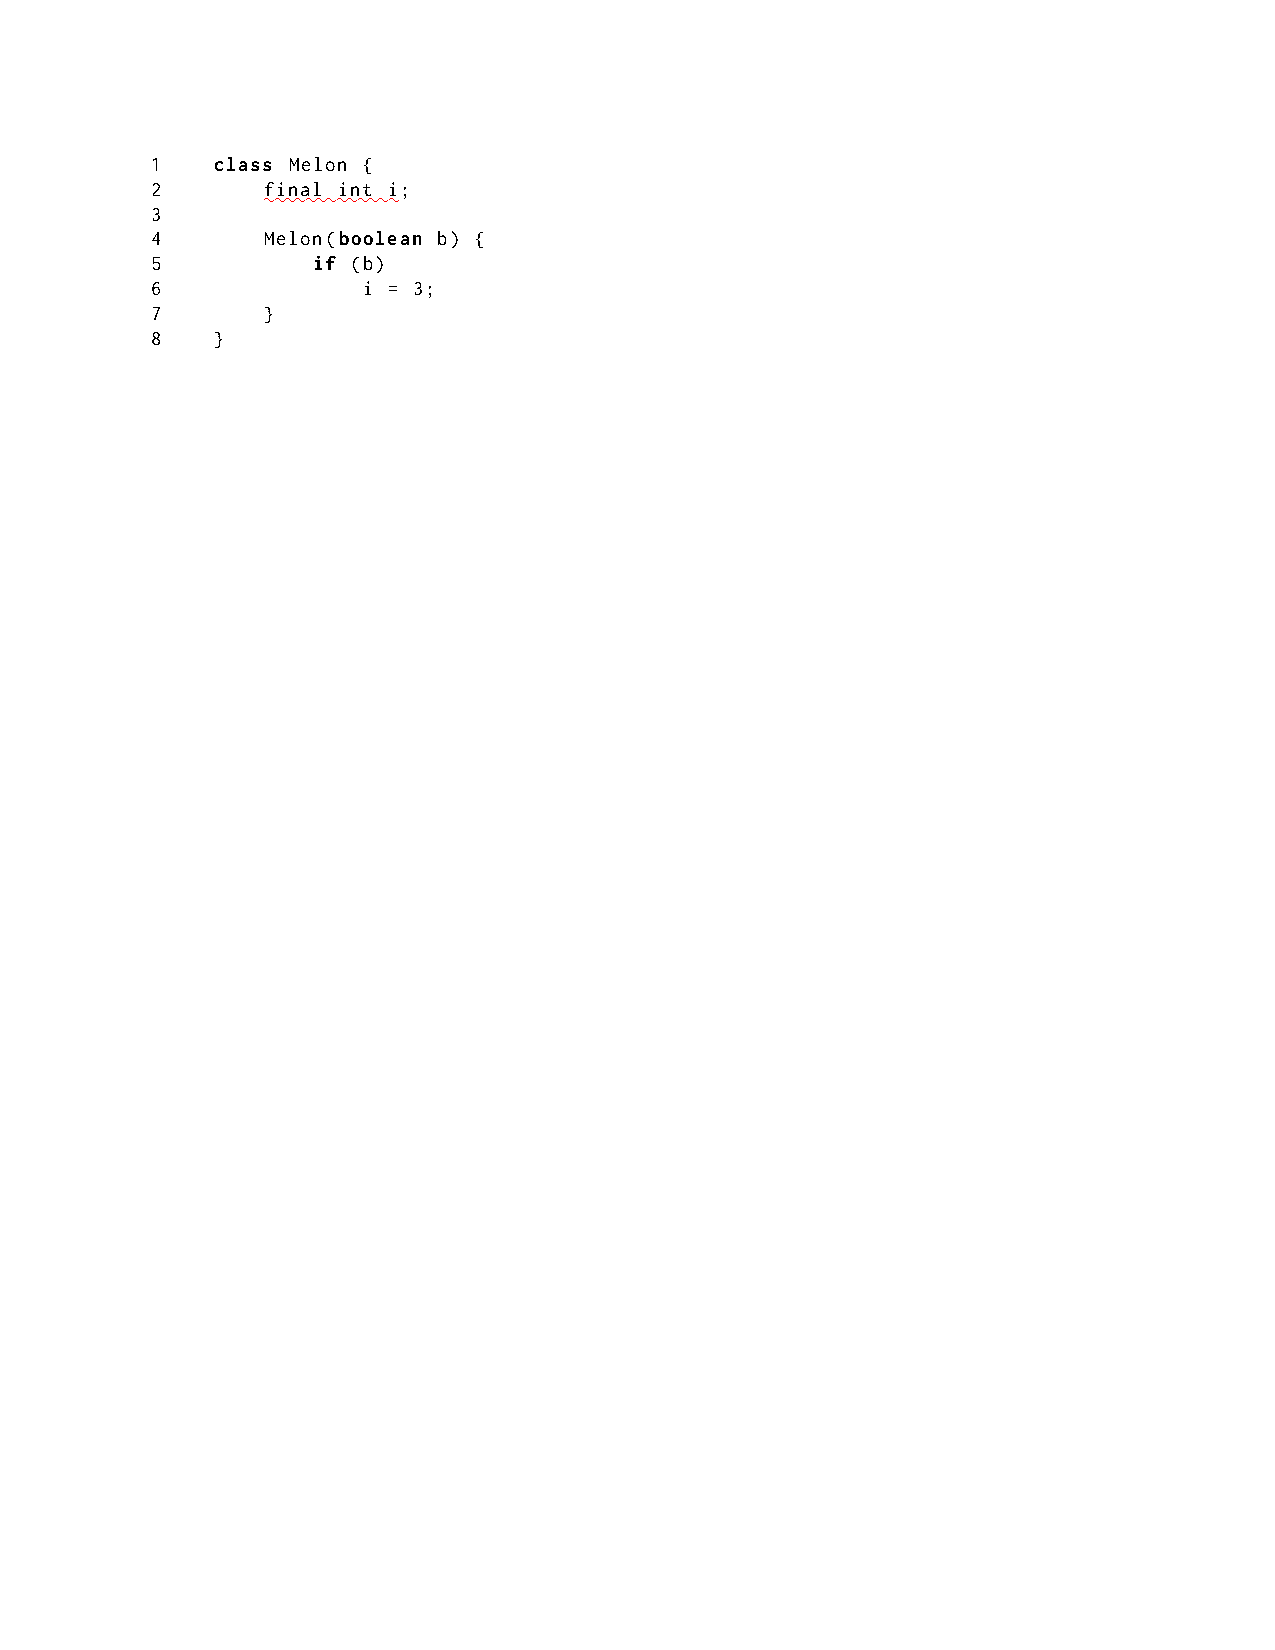
\includegraphics{melon_wavy_crop}}
  \\
  % \vspace{0.2cm}
  \subfloat[Explanatory visualization\label{fig:melon:explanatory}]
    {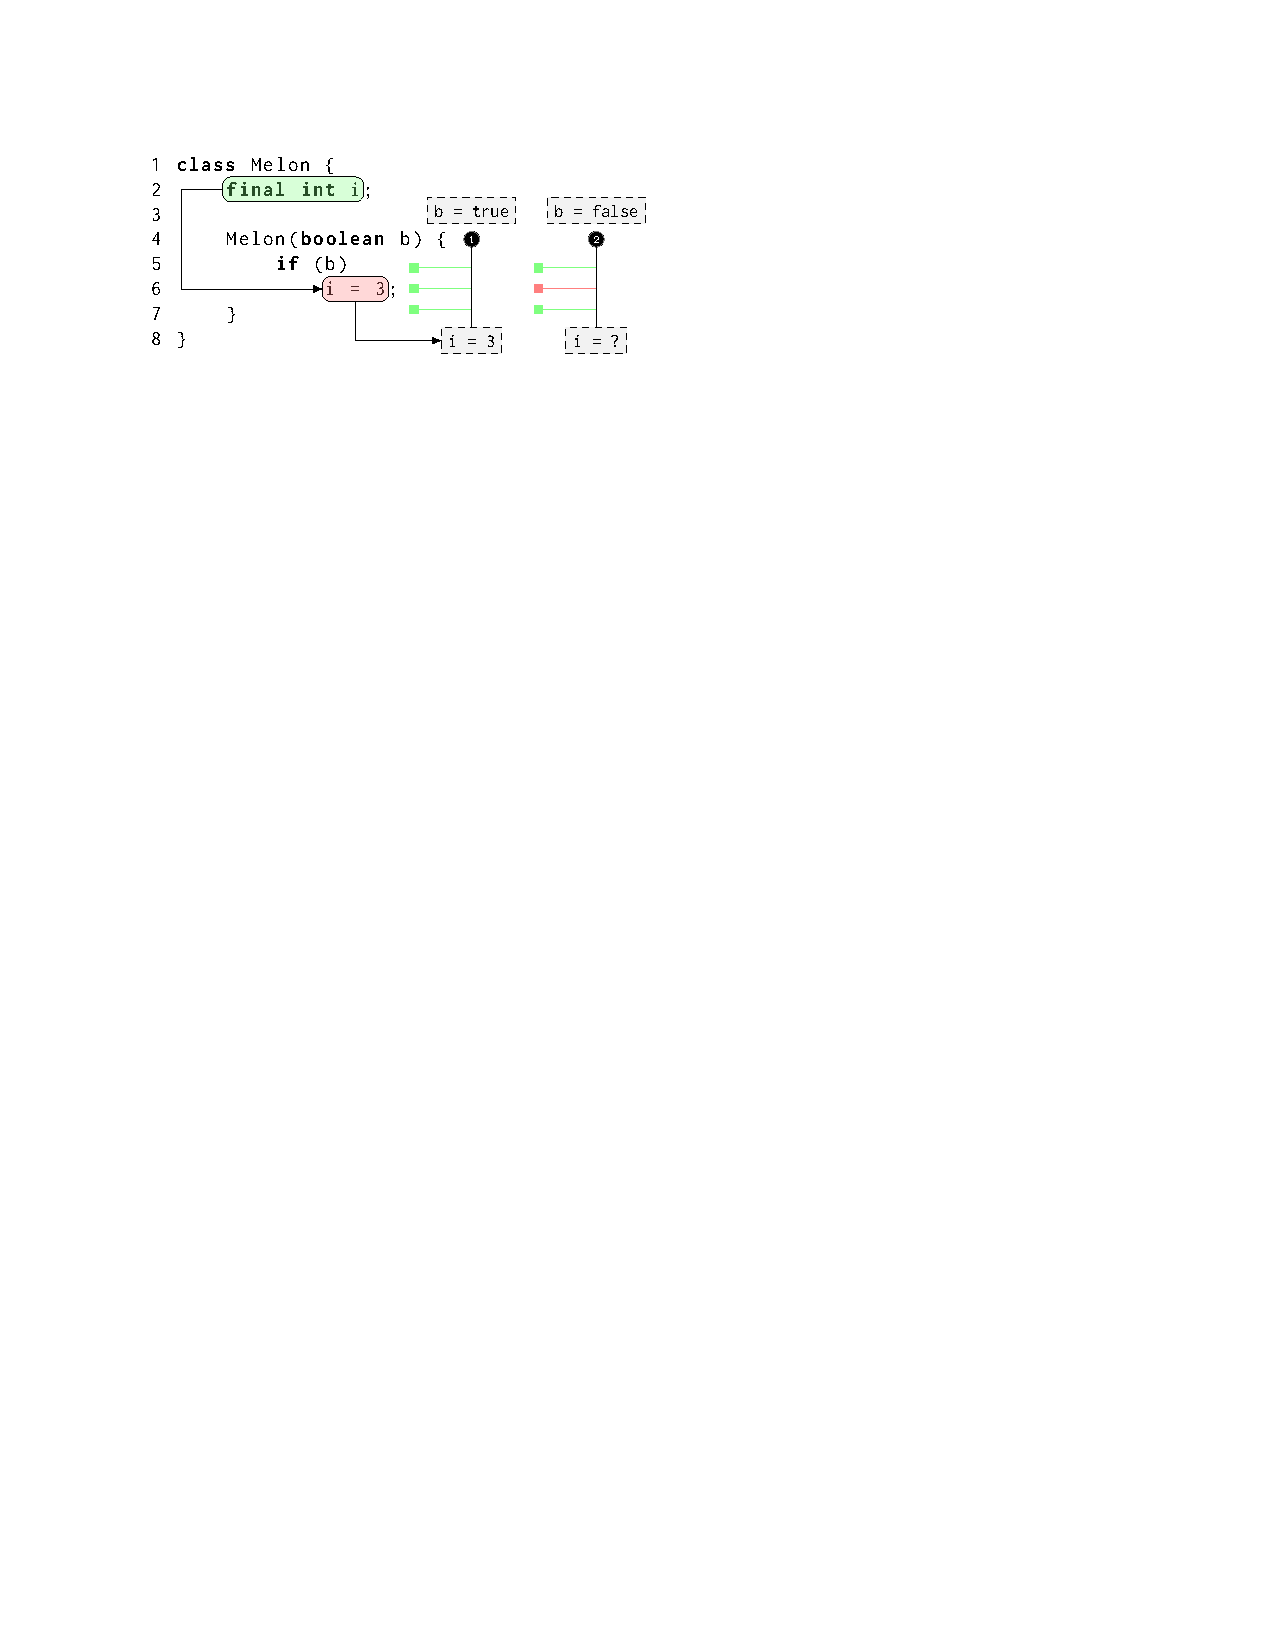
\includegraphics{melon_explain_crop}}
  \\
  \subfloat[Error message text\label{fig:melon:text}]{\usebox{\melonlisting}}
  \caption{A comparison of a potentially uninitialized variable compiler error through (a) baseline visualizations, the dominant paradigm as found in IDEs today, (b) our explanatory visualizations, and (c) the textual error message.\label{fig:melon}}
\end{figure}

Modern integrated development environments (IDEs), such as Eclipse, IntelliJ, and Visual Studio, offer a number of visualizations to assist developers in more effectively identifying and comprehending compiler error notifications. For example, in addition to the full error message text found in an output or dedicated error window, such notifications may include an indicator in one or more margins, along with a red wavy underline visualization overlaid on the source text to indicate a relevant location of the error.

% The IDE may also use tooltips, visual popups containing a textual error description; these are activated when the mouse hovers over the red wavy underline visualization.

Many developers consider these error notifications to be cryptic and confusing~\cite{Traver2010}. We postulate one of the reasons error notifications are confusing for developers is because compilers use a sophisticated reasoning process to determine that an error exists in the source code, but do not reveal this reasoning process to either the IDE or the developer.

More explicitly, in order to generate an error notification, the compiler begins with the source code, collects information during its compilation, uses that information to identify that a problem exists, and notifies the developer of the problem through the IDE. Yet, for developers to comprehend the notification, they must mentally duplicate this process through \textit{self-explanation}~\cite{Parnin2011} in essentially reverse order --- starting with the error notification, the developer must identify what they think the problem might be from the IDE's presentation, mentally collect all of the program components related to this problem, and finally identify the area or areas of source code necessary to correct the particular defect. This self-explanation process, when left solely to the developer, can result in a significant loss of productivity because humans are imperfect and bounded in knowledge, attention, and expertise~\cite{Ko2005}. \textit{But much of this self-explanation process may be completely unnecessary since the reasoning process that resulted in the error notification was already known to the compiler.}\footnote{As Bret Victor points out his talk ``Inventing on Principle'' (CUSEC 2012): ``If we're writing our code on a computer, why are we simulating what a computer would do in our head? Why doesn't the computer just do it, and show us?''}

Visualizations in IDEs, such a red wavy underlines and margin indicators, take the perspective that compilers are \textit{opaque} black boxes, and thus by design are limited in their affordances for helping developers in comprehending error notifications. In this paper, we argue that developers stand to significantly benefit when compilers are made more \textit{transparent} and expose their internal reasoning process to visualization systems. We argue that such systems can leverage these structures to generate expressive, \textit{explanatory visualizations} that align with the way in which developers self-explain error notifications. Our contributions in this paper are:

\begin{itemize}
\item A foundational set of composable visual annotations that aid developers in better comprehending error messages.
\item An \textit{explanation task} evaluation, using a set of paper mockups, which demonstrates that our explanatory visualizations yield more correct self-explanations than the baseline visualizations used in IDEs today. These annotations are used intuitively by developers in their own self-explanations of error messages, even when explanatory visualizations have not been provided to them.
\item A \textit{recall task} evaluation, in which developers write programs that intentionally generate compile errors, which demonstrates that better self-explanations enable developers to construct better mental models of error notifications.
\end{itemize}

\section{Motivating Example}

Yoonki is an experienced C++ developer who has recently transitioned to a project that is being developed in the Java programming language. While programming, he encounters a wavy red underline visualization as shown in Figure~\ref{fig:melon:base}, which indicates an error. The problem seems to be related to \texttt{final int i}, which Yoonki recognizes as being roughly similar to the concept of a \texttt{const} variable in C++. Yoonki investigates further and notices the full text of the error in the bottom pane of his IDE (Figure~\ref{fig:melon:text}). 

However, Yoonki is now a bit puzzled. The error message indicates that the variable might not be initialized at Line 7. He chooses to ignore this error message as being incorrect because Line 7 contains only a curly brace, which seems to have nothing to do with his problem. He is comfortable in doing so because in C++, he often received unhelpful notifications.

Yoonki explains to himself that the problem is that \texttt{final} variables in Java, like \texttt{const} variables in C++, must be initialized at their point of declaration, or in a constructor initializer list. Satisfied with his explanation, he rewrites Line 2 to read \texttt{final int i = 3;}, but this immediately results in a downstream error, as Line 6 now returns \texttt{cannot assign a value to final variable i}. Yoonki realizes that a constant cannot be re-assigned, so he deletes the entire conditional statement. Even though the program now compiles, the fix happens to be an incorrect one.

The problem here is that Yoonki has learned a reasonable heuristic for how constant variables work in programming languages, but his heuristic fails in this case. Like C++, Yoonki is correct in that Java \texttt{final} variables can only be assigned once. But unlike C++, \texttt{final} variables in Java can be assigned at a point other than the declaration. Yoonki has experienced what we could call a \textit{knowledge breakdown}~\cite{Ko2005}. In this case, Yoonki has a confirmation bias about how the system is supposed to work, and this false hypothesis has worked reasonably well for him until now.

This false hypothesis remains uncorrected by the IDE. In his IDE, the red wavy underline visualization can only indicate a single location related to the error. The IDE is unable to convey that the problem is dependent on several program elements. For example, the error text and the indicated location is accurate in that after this line the variable might be uninitialized, but the IDE does not have an effective way to indicate how that location relates to the \texttt{final} variable.

In contrast, consider our approach, shown in Figure~\ref{fig:melon:explanatory}. Here, Yoonki may not experience the same knowledge breakdown, because the IDE provides a visual explanation of the problem within his source code. Though Yoonki might once again incorrectly assume that \texttt{final} variables must be initialized at declaration, the visualization implies that the problem is actually related to control flow. Specifically, the explanatory visualization is showing Yoonki that there is a code path in which \texttt{i} is assigned a value (when \texttt{b = true}), and another code path where it is not (when \texttt{b = false}). This time, Yoonki correctly fixes the defect by adding an \texttt{else} statement to the condition, initializing it with an appropriate value in the case when \texttt{b = false}.

This hypothetical scenario illustrates why the dominant visualization paradigm is not sufficient in supporting the process of self-explanation. As we argue in this paper, this scenario is illustrative of the more general problem with the output of program analysis tools: these tools present only the end-result of the reasoning process and therefore do not support the developer in self-explaining.

\section{Pilot Study}
\label{sec:pilotstudy}

\begin{table}[!t]
\caption{Frequency of Visual Annotations in Pilot\label{tab:pilot}}
\centering
\begin{tabularx}{\columnwidth}{lrX}
\toprule
Annotation & Frequency & Description\\
\midrule
Point & 49 & Indicates that a particular token or set of tokens has been marked. Examples include underlining or circles the token(s).\\
[0.2cm]
Text & 45 & Indicates natural language text. For example, ``assign a value to the variable'' or ``dead code''.\\
[0.2cm]
Association & 33 & Indicates an association between two or more program elements, which is accomplished by drawing a connecting line between the elements, with or without arrow heads.\\
[0.2cm]
Symbol & 20 & Symbols include visual annotation such as \texttt{?} or \texttt{x}, or numbered circles, to name a few.\\
[0.2cm]
Code & 14 & Explanatory code that is written in order to explain the error message, for example, \texttt{if (b == false)} or \texttt{m(1.0, 2)}. This does not have to be correct Java code, but should be interpretable as pseudocode.\\
[0.2cm]
Strikethrough & 5 & The strikethrough is separated from the point annotation because this annotation is provided by IDEs today, and has pre-established semantics.
\\
[0.2cm]
Multicolor & - & The use of more than a single color to explain a concept. For example, green may be used to indicate lines that are okay, and red to indicate lines that are problematic. This option was not available to students in the pilot study.\\
[0.2cm]
\bottomrule
\end{tabularx}
\end{table}

We conducted a pilot study\footnote{All experimental study materials are available at \url{http://go.barik.net/errviz}.} from undergraduate lab sessions in Software Engineering to address a pre-requisite research question:
\begin{description}
\item[\textbf{RQ0}] What annotations do developers use when they explain error messages to each other?
\end{description}

We hypothesized that if participants preferred certain types of annotations when explaining error messages to each other, they could also benefit when the same annotations were used to explain error messages to them through their IDE.

Thus, before generating our annotations, we conducted an informal lab activity with third-year Software Engineering students. Each student was given a sheet of paper with a source code listing and the corresponding compiler error message. The source code listings were unadorned and lacked any visual annotations.

Students were paired in order to perform an explainer-listener active learning exercise. This is an exercise in which one student, the explainer, is asked to verbally explain the error message to the other student, while visually annotating the source code listing during their explanation. Access to external materials was not allowed. After two minutes of explanation, roles were swapped and the second explainer annotated the second error message.

We randomly assigned one of four source code listings to each student, pulled verbatim from the OpenJDK 7 unit tests for compiler diagnostics framework. These examples, among others used in subsequent studies, are found in Table~\ref{tab:tasks}, and no students within a pair received the same source code listings. In total, we collected 73 samples:  17 from T1 (23\%), 12 from T2 (16\%), 20 from T3 (27\%), and 24 from T6 (33\%). Students did not receive tasks T4 or T5, because they had not been created at the time of the pilot study.

From these annotations, we performed two passes over the student responses. In the first pass, we created a taxonomy of visual annotations based on our observations. In the second pass, we classified the student responses using this taxonomy. The aggregated results are shown in Table~\ref{tab:pilot}.

Our own explanatory visualizations are informed by this pilot study, through which we implement annotations such as points, associations, symbols and explanatory code. Since students used these types of annotations without any \textit{a priori} prompting, we postulate that they find these types of annotations intuitive to use during explanation.


\section{Explanatory Visualizations of Error Messages}
\label{sec:motivation}

\begin{table}[!t]
\caption{Visual Annotation Legend\label{tab:viztax}}
\centering

\renewcommand{\tabularxcolumn}[1]{m{#1}}
\begin{tabularx}{\columnwidth}{m{0.4in}X}
\toprule
Symbol & Description\\
\midrule

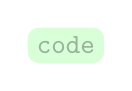
\begin{tikzpicture}
\node[opacity=0.3,fill=green!50,rounded corners,text=black] at (0,0) { \texttt{code} } ;
\end{tikzpicture} 
& Indicates the starting location of the error.\\\\

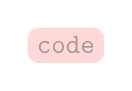
\begin{tikzpicture}
 \node[fill opacity=0.3,fill=red!50,rounded corners] 
    at (0,0) { \texttt{code} };
\end{tikzpicture} & Indicates issues related to the error.\\\\

\begin{tikzpicture}
\draw[>=latex,->] (0,0) -| (1em, 1em );
\end{tikzpicture}  & Arrows can be followed. They indicate the next relevant location to check.\\\\


\begin{tikzpicture}
 \node[circle,draw=gray,very
    thin,fill=black,text=white,inner sep=1pt] at (0,0) {\tiny 1};
\end{tikzpicture} & Enumerations are used to number items of potential interest, especially when the information doesn't fit within the source code.\\\\

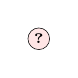
\begin{tikzpicture}
\node (node 1) at (0,0) [circle,draw=gray,very
    thin,fill=red!10,text=white,inner sep=1pt,draw=black,text=black] at (0,0) {\tiny \textbf{?}};
\end{tikzpicture} & The compiler expected an associated item, but cannot find it.\\\\


\begin{tikzpicture}
  \node[draw=red,cross out,inner sep=2pt,fill=black,text=white,thick] at (0,0) {};
\end{tikzpicture} & Indicates a conflict between items.\\\\

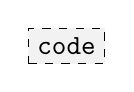
\begin{tikzpicture}
\node[draw,rectangle,draw=black,fill=gray!10,dashed,right] at (0,0) {\texttt{code}};
\end{tikzpicture} & Explanatory code or code generated internally by the compiler. The code is not in the original source.\\\\

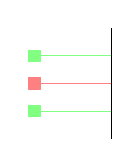
\begin{tikzpicture}
\draw (0,0) -- (0,-4em);
\draw[>=square,->,draw=green!50,fill=green!50]    
      (0,-1em) -- +(-3em, 0em);
  \draw[>=square,->,draw=red!50,fill=red!50]
    (0,-2em) -- +(-3em, 0em);
  \draw[>=square,->,draw=green!50,fill=green!50] 
    (0,-3em) -- +(-3em, 0em); -- +(-3em, 0em);
\end{tikzpicture} & Indicates code coverage. Green lines indicate successfully executed code. Red lines indicate failed or skipped lines.\\

\bottomrule
\end{tabularx}
\end{table}
\renewcommand{\tabularxcolumn}[1]{p{#1}}

We propose a set of eight visual annotations, which are summarized in Table~\ref{tab:viztax}. We now concretely describe these annotations using the motivational example from Figure~{\ref{fig:melon:explanatory}}. The starting \emph{point} for visual explanation in the source code listing is indicated using 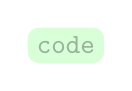
\begin{tikzpicture}[baseline=-0.5ex]
\node[opacity=0.3,fill=green!50,rounded corners,text=black] { \texttt{code} } ;
\end{tikzpicture} (a green rectangle with rounded corners that surrounds a program element). In our visualization mockups, we choose the starting point to be the same as the source of the error identified by IntelliJ (Figure~\ref{fig:melon:base}). In the example, this is \texttt{final int i}.

Continuing our example, the starting point is associated with a second point, \texttt{int i}, because this is where the potential assignment to the variable occurs. We indicate this with 
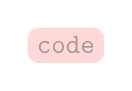
\begin{tikzpicture}[baseline=-0.5ex]
\node[opacity=0.3,fill=red!50,rounded corners,text=black] { \texttt{code} };
\end{tikzpicture} (red rectangle with rounded corners), and the association is indicated by 
\begin{tikzpicture}
\draw[>=latex,->] (0,0) -| (1em, 1em );
\end{tikzpicture} (a directional arrow).

A second association leads the developer to an explanatory code block that copies the statement. Explanatory code is represented by
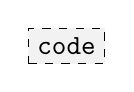
\begin{tikzpicture}[baseline=-0.5ex]
\node[draw,rectangle,draw=black,fill=gray!10,dashed,right] at (0,0) {\texttt{code}};
\end{tikzpicture} (dashed gray rectangle), which indicates that the surrounded elements are explanatory and not part of the original source code of the program. This explanatory code block is part of a larger \textit{composite annotation} describing the control flow scenario under which the statement is executed.

This composite annotation demonstrates that several basic annotations can be combined to create a new annotation for expressing a more complex concept. One of these components is the code coverage annotation. This annotation uses
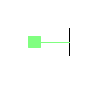
\begin{tikzpicture}
\draw (0,0) -- (0,-1em);
\draw[>=square,->,draw=green!50,fill=green!50]    
      (0,-0.5em) -- +(-1.5em, 0em);
\end{tikzpicture} (green line) and 
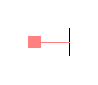
\begin{tikzpicture}
\draw (0,0) -- (0,-1em);
\draw[>=square,->,draw=red!50,fill=red!50]    
      (0,-0.5em) -- +(-1.5em, 0em);
\end{tikzpicture} (red line) to indicate whether or not a line is covered. In addition, the enumerations 
\begin{tikzpicture}
 \node[circle,draw=gray,very
    thin,fill=black,text=white,inner sep=1pt] at (0,0) {\tiny 1};
\end{tikzpicture} and 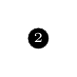
\begin{tikzpicture}
 \node[circle,draw=gray,very
    thin,fill=black,text=white,inner sep=1pt] at (0,0) {\tiny 2};
\end{tikzpicture} provide the developer with convenient labels for referring to the branches (for example, ``It looks like it works fine in branch 1, but not in branch 2''). The final component is another explanatory code block indicating one possible condition under which the branch would be executed.

Thus, the composite annotation indicates that \texttt{i = 3}, and all statements within branch 1 will be executed when \texttt{b = true}. This composite annotation is then used to show the developer a counterexample in which \texttt{i} would be uninitialized. A simple text explanation stating that \texttt{i is uninitialized when b = false} would have provided the same conclusion, but we hypothesize that the intermediate steps in the explanation are important for developer comprehension.

There are two visual annotations that do not appear in the motivating example that warrant explanation. These are 
\begin{tikzpicture}
  \node[draw=red,cross out,inner sep=2pt,fill=black,text=white,thick] at (0,0) {};
\end{tikzpicture} (red cross), which indicates that a conflict exists between blocks, such as when the developer accidentally specifies repeated modifiers:

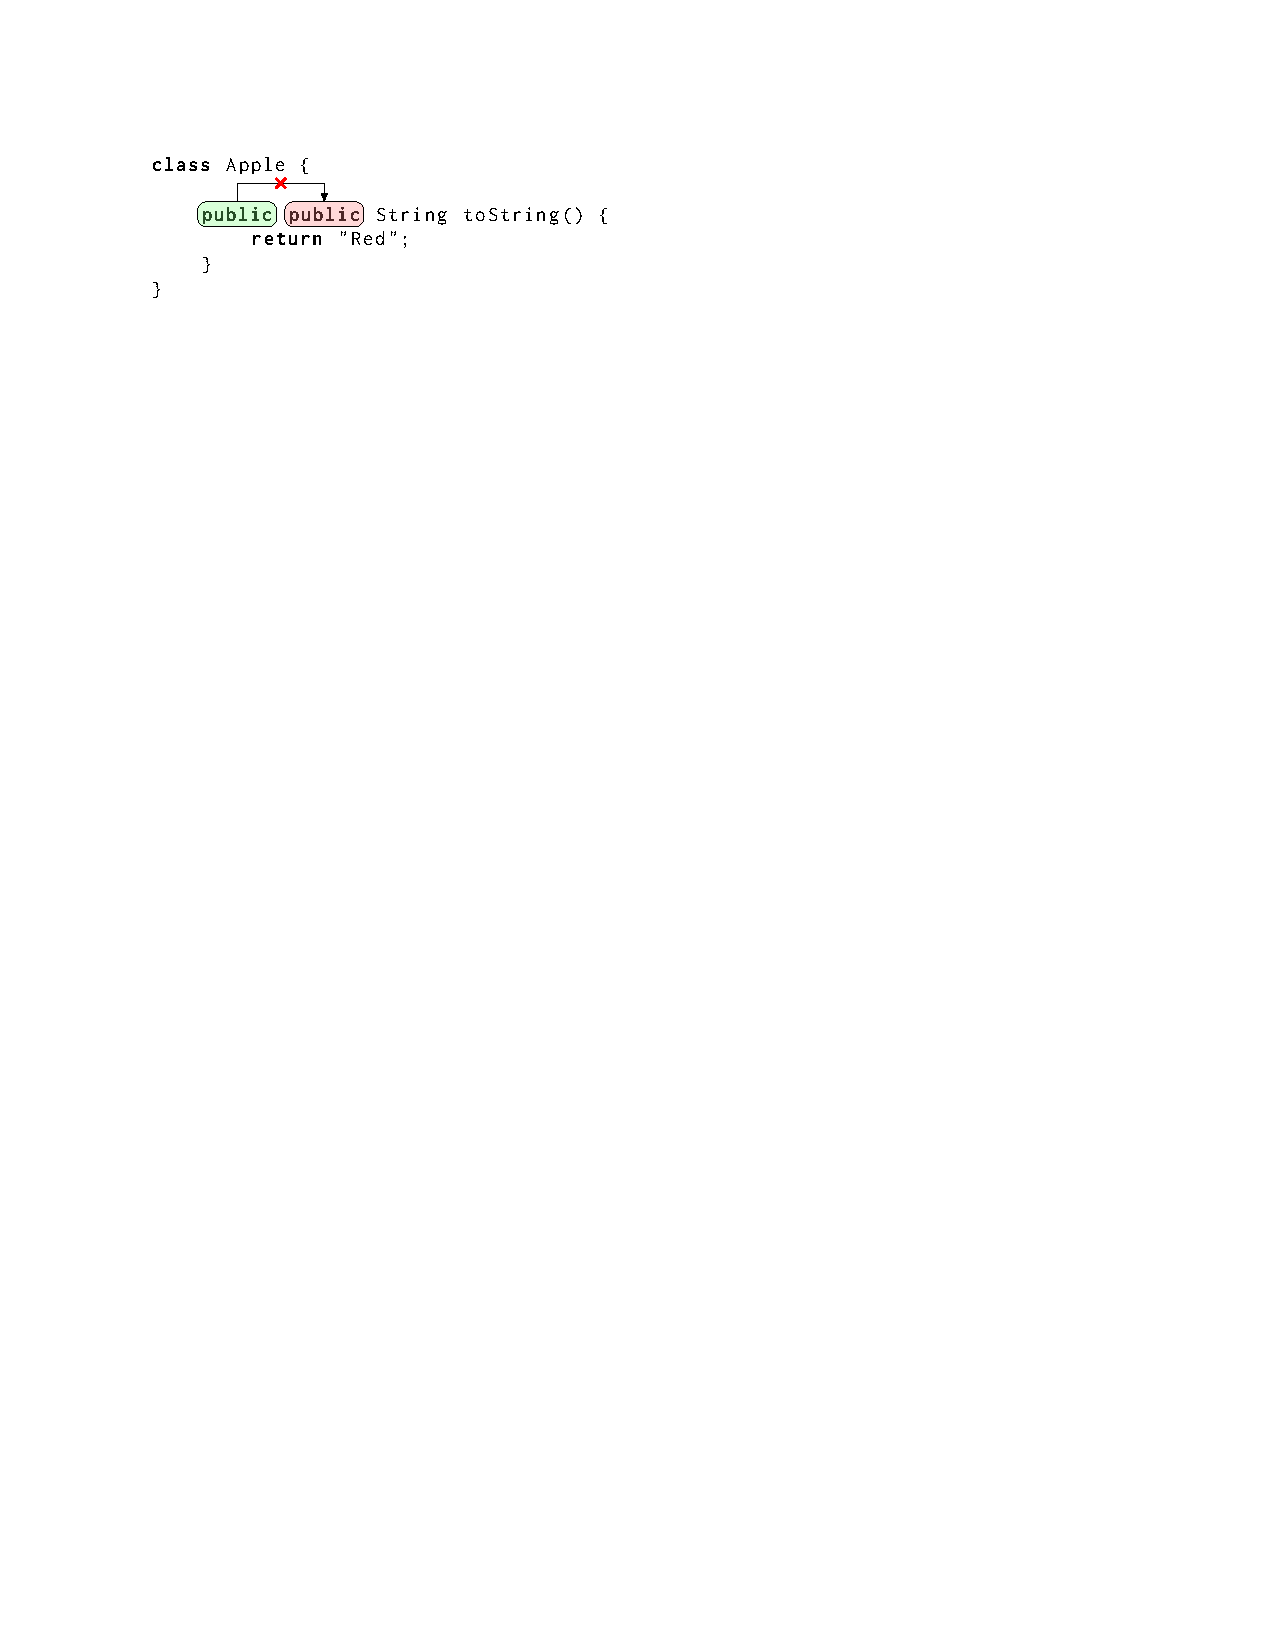
\includegraphics{apple_explain_crop.pdf}

Finally, the 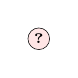
\begin{tikzpicture}
\node (node 1) at (0,0) [circle,draw=gray,very
    thin,fill=red!10,text=white,inner sep=1pt,draw=black,text=black] at (0,0) {\tiny \textbf{?}};
\end{tikzpicture} is used to indicate that the program element should be associated with another element, but that the connecting element is not found. This can occur, for example, when a \texttt{catch} statement is unreachable either because the exception can never be thrown, or because it is always caught by a prior \texttt{catch} clause:

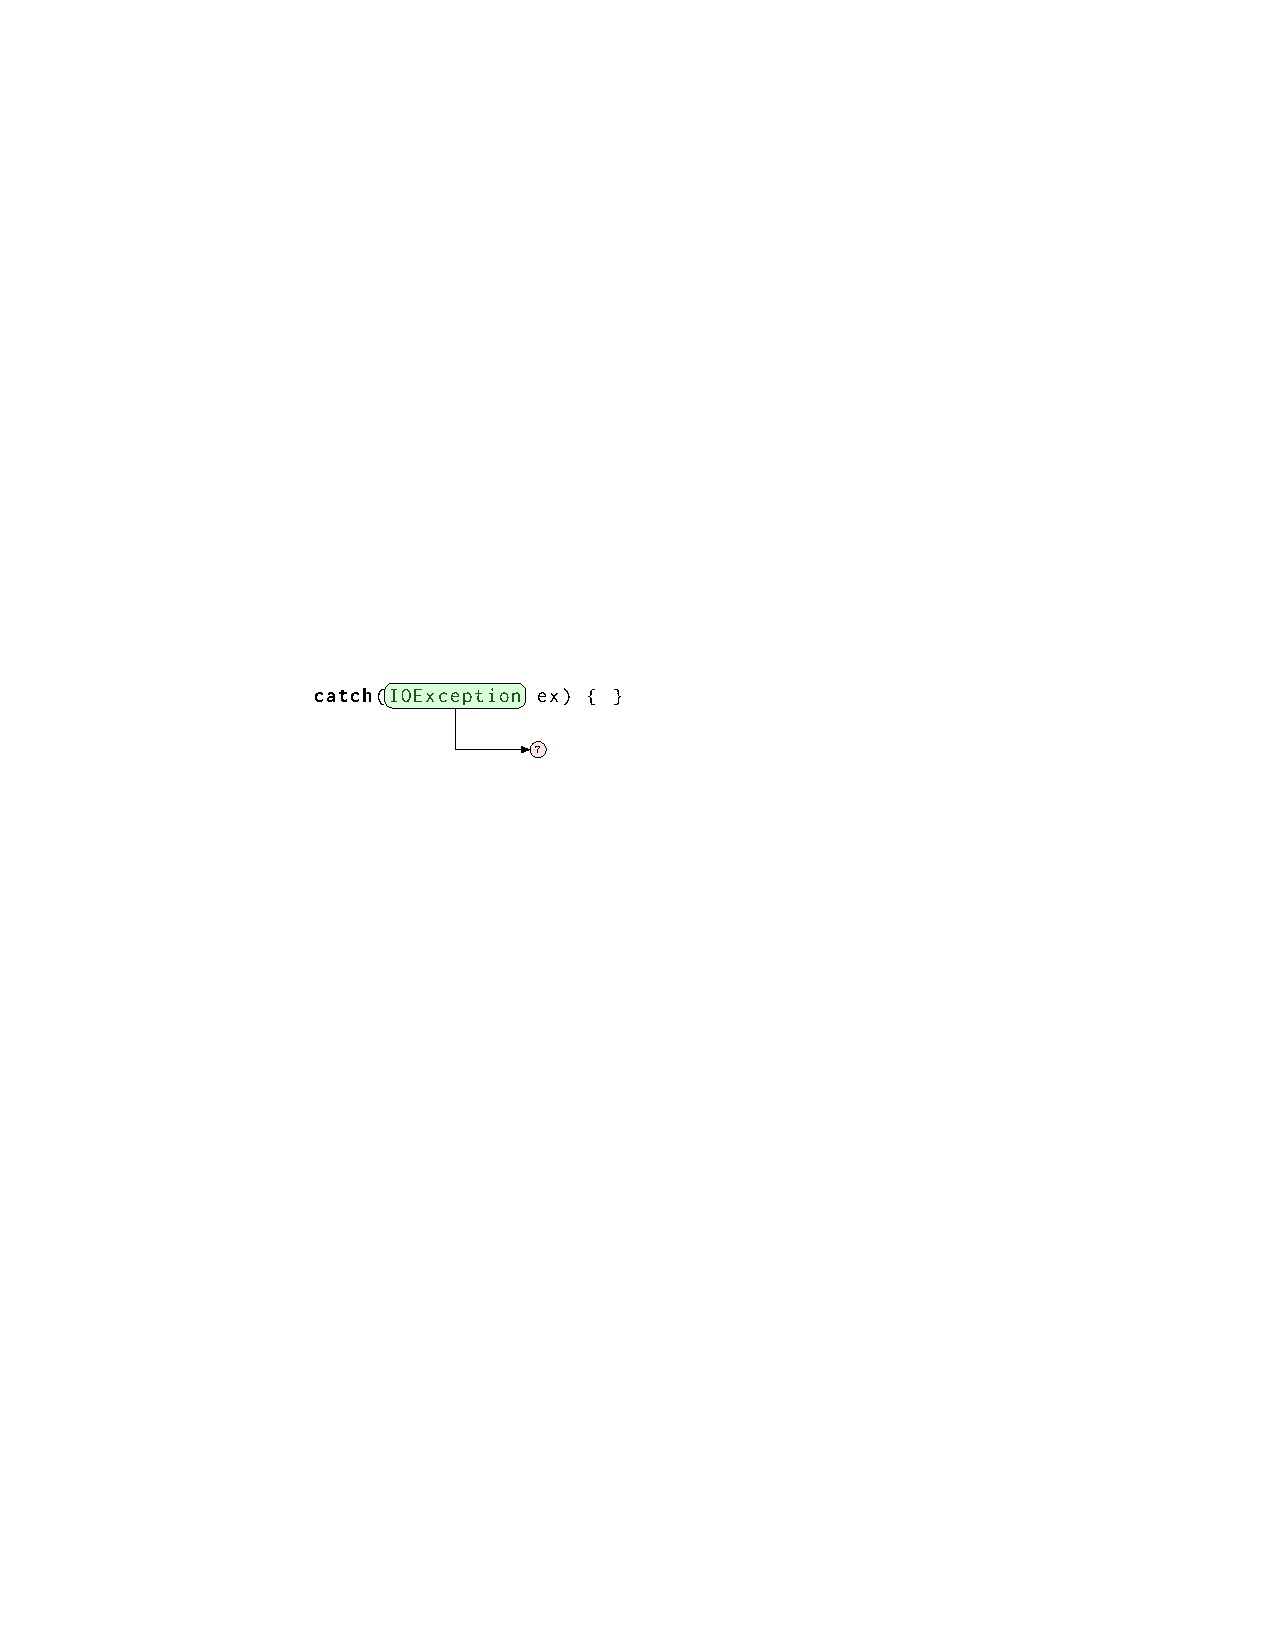
\includegraphics{trumpet_explain_crop.pdf}

\section{Methodology}

We conducted a second, formal study, which we discuss for the remainder of this paper.

\subsection{Research Questions}

Broadly, we assigned participants randomly to two groups: a control group, having access to the baseline visualization (red wavy underline) in their source code, and a treatment group, having access to our explanatory visualizations. We designed our experiment to elicit answers for four research questions:

\begin{description}
\item[\textbf{RQ1}] Do explanatory visualizations result in more correct self-explanations by developers?
\item[\textbf{RQ2}] Do developers adopt conventions from our visual annotations in their own self-explanations?
\item[\textbf{RQ3}] What aspects differentiate explanatory visualizations from baseline visualizations?
\item[\textbf{RQ4}] Do better self-explanations enable developers to construct better mental models of error notifications?
\end{description}

Unlike the baseline visualization, explanatory visualizations are intended to expose the reasoning process of the compiler. 

For RQ1, we hypothesized that exposing this reasoning process would result in significantly more correct explanations by developers. If this hypothesis was not supported, then it would imply that the explanatory visualizations may be confusing to developers, and that developers reason about error messages in a very different way than our diagrammatic representation.

For RQ2, we hypothesized that both the control group and treatment group would adopt similar annotations when developers explained error messages, because our visualizations are based on conventions that developers would find intuitive for self-explanation.

For RQ3, we wanted to identify the traits of the explanatory visualizations beneficial to developers in comprehending error notifications. Significant differences in traits between the baseline visualization and explanatory visualizations would give us insight into the design of explanatory visualizations in general.

For RQ4, we hypothesized that better explanations result in better mental models, and that developers with explanatory visualizations would have a significantly higher frequency of better mental models than the control group.

\subsection{Participants}

We recruited 28 participants ($n = 28$) from a third-year undergraduate course in Software Engineering. We offered participants extra credit on their final exam for participating in the study. Participants self-reported demographic data. Five of the participants were female (17.8\%). The mean age of the participants was 22 ($s = 3.6$). Participants reported a mean of 9 months ($s = 12$) of industry programmer experience.

% We further identified outliers through quartile construction to find the standard deviation attributable to three participants self-reporting 28 months, 40 months, and 48 months of experience. Without these participants, the mean industry programmer experience is 5 months ($s = 6$). We performed all analyses with and without these outliers. We concluded that the high outliers were otherwise unremarkable except in their self-reporting and therefore we gave no special consideration to them in subsequent reporting within this paper.

Participants reported using the Eclipse IDE as their primary Java programming environment; two participants reported IntelliJ. On a 4-point Likert-type item scale of \emph{Novice---Expert}, 13 participants reported their overall programming ability as Intermediate (46\%), 14 as Advanced (50\%), and 1 as Expert (4\%). No participants ranked themselves as Novice. On a 4-point scale \emph{Not knowledgeable---Very knowledgeable}, 19 participants indicated they they were knowledgeable about Java (68\%), and the remaining 9 participants indicated that they were very knowledgeable about Java (32\%).

% \subsection{Methodology}

% http://www.real-statistics.com/non-parametric-tests/mann-whitney-test/


% this is a non-random sampling of error messages.

% How to Report Mann-Whitney U: http://yatani.jp/HCIstats/MannWhitney
% "Median latencies in groups E and C were 153 and 247 ms; the distributions in the two groups differed significantly (Mann–Whitney U = 10.5, n1 = n2 = 8, P < 0.05 two-tailed)."

\subsection{Selection Criteria for Mockups}

\begin{table*}[!t]
\caption{Participant Explanation and Recall Tasks\label{tab:tasks}}
\centering
% Some packages, such as MDW tools, offer better commands for making tables
% than the plain LaTeX2e tabular which is unsolved here.
\begin{tabularx}{\textwidth}{lllX}
\toprule
Task Order & Task Name & OpenJDK File & Error Message\\
\midrule

T1 & Melon & \texttt{VarMightNotHaveBeenInitialized.java} & \texttt{variable i might not have been initialized} \\
[0.2cm]
\midrule

T2 & Kite & \texttt{UnreportedExceptionDefaultConstructor.java} & \texttt{unreported exception Exception in default constructor} \\
[0.2cm]
\midrule

T3 & Brick & \texttt{RefAmbiguous.java} & \texttt{reference to m is ambiguous, both method m(int,double) in Brick and method m(double,int) in Brick match}\\
[0.2cm]
\midrule

T4 & Zebra & \texttt{InferredDoNotConformToBounds.java} & \texttt{cannot infer type arguments for BlackStripe<>;\newline
reason: inferred type does not conform to declared bound(s)\newline\newline
inferred: String\newline
    bound(s): Number}\\
[0.2cm]
\midrule

T5 & Apple & \texttt{RepeatedModifier.java} & \texttt{repeated modifier
}\\
[0.2cm]
\midrule

T6 & Trumpet & \texttt{UnreachableCatch1.java} & \texttt{unreachable catch clause\newline     
  thrown types FileNotFoundException,EOFException have already been caught
}\\
[0.2cm]

\bottomrule
\end{tabularx}
\end{table*}

For our study, we decided to use undergraduate students because they are readily available and because we wanted to reserve our more limited industry participants for a full implementation. Because our University requires students to have knowledge of the Java, we selected examples in this language to mockup our visualizations.

Pragmatically, we wanted to keep our entire study under an hour, and due to this experimental design constraint could only present six novel visualizations to participants. We readily admit that the selection of these visualizations was not random, and offer our justification for this decision here. 

We selected our compiler error examples from the OpenJDK diagnostics framework.\footnote{The framework contains a sample source code listing for almost every compiler error within Java. The source files may be downloaded at \url{http://hg.openjdk.java.net/jdk7/tl/langtools/}, and then by browsing to \texttt{test/tools/javac/diags/examples/}.} This framework contains a collection of 382 Java code examples, each of which is designed to generate one or more error messages when compiled.

Since some error messages may be more conceptually sophisticated than others (for example, ``illegal escape character'' is not particularly suited to an explanatory visualization), we hand-selected a set of examples that we believed could benefit most from visual annotations. If no significant results could be identified even from this hand-selected set, then it would suggest that this visualization is not worth pursuing for a full implementation.

Furthermore, our visualization system is not intended to teach new concepts; rather, it is intended to aid the developer in understanding how a particular instance of an error message applies to a specific source file. Consequently, we selected examples based on concepts that students were expected to already know from their coursework, such as constants and variables, exceptions, and classes.

% participants must already know the underlying concepts, though the visual annotations may sometimes force the participant to reconcile their incorrect understanding of the error message when their interpretation conflicts with the visual annotations presented by the tool.

Ultimately, we selected messages that we believed could effectively demonstrate the rich explanatory potential of visualizations, while balancing the capability of the participants. The selected messages are summarized in Table~\ref{tab:tasks}.

\subsection{Mockup Construction Procedure}

Using the six selected error messages, we constructed a total of 12 mockups --- six for the the control group, and six for the treatment group. The paper mockups were designed to resemble how the visualization would appear within the text editor of the IDE, with one mockup per page. Each page contained a listing of the source code with the appropriate visualizations and line numbers. The code listing was followed by the text of the compiler error message.

The control group mockups were designed by directly copying the red wavy underline visualizations provided by the IntelliJ IDE for the Java code examples. IntelliJ also provides interactive tooltips for each error, which are shown when the developer hovers over an annotated substring. However, we did not consider these interactive features since we are specifically interested in the contribution of the explanatory capability of the non-interactive visualizations. We chose IntelliJ over the Eclipse IDE because it uses the same text error messages as the command-line OpenJDK compiler, which is important to our experimental design.

The treatment group mockups were informed by a pilot study through which we elicited an initial taxonomy of visual annotations that appeared to be useful to developers when they explained concepts to other developers (for details of this elicitation process, see Section~\ref{sec:pilotstudy}). We used the annotations from this pilot experiment as a foundation to  manually draw visual annotations for six of the error messages. 
We used our own experiences with compiler technologies, such as Roslyn\footnote{\url{http://msdn.microsoft.com/en-us/library/roslyn.aspx}}, to render visualizations that we think are plausible for compilers to render if they expose the appropriate data structures to a visualization system.

% For purposes of our study, we also assumed the existence of algorithms that reasonably manage layout issues when visualizations are overlaid on text. This assumption is not entirely unfounded, as we implemented our renderings using TikZ and PGF for LaTeX, a graphics system which provides some support for placing and routing diagrams over text.

% BEGIN ZEBRA FIGURE
% ==================
\newsavebox{\zebralisting}
\begin{lrbox}{\zebralisting}
\begin{lstlisting}[style=JavaError]
Zebra.java:8: error: cannot infer type arguments for BlackStripe<>;
   Stripe<String> sf1 = new BlackStripe<>("Marty");
                        ^
  reason: inferred type does not conform to declared bound(s)
    inferred: String
    bound(s): Number
1 error
\end{lstlisting}
\end{lrbox}

\subsection{Investigator Training}

The first and second authors conducted the experiments. To increase consistency between the authors, the first author conducted a practice session with the second author acting as a participant. We then reversed the roles, and the study was repeated. Through this process, we developed a formal protocol script for conducting the sessions.

\subsection{Experimental Procedure}

% Schnidermann did a study with nonprogrammers and programmers to see if programmers were better able to reproduce code listings, indicating that programmers semantically remember code.  We based our study off of Schnidermann's by designing our study with two secions -- a recognition section and a recall section.

\subsubsection{Assignment}
We randomly assigned participants to one of two groups --- control or treatment, such that each group had an equal number of participants. This resulted in 14 participants per group. The only difference between the treatment and control groups was the type of visualizations that they used during the experiment.

\subsubsection{Recording}
Participants filled out an informed consent form and indicated whether or not they wanted their audio and screens to be recorded. For participants who agreed to be recorded ($n=26$), we used desktop recorder software to record both the audio of the explanations as well as screen interactions during the experiment.

\subsubsection{Phase 1: Self-Explanation Phase}

% \begin{figure*}[!t]
%   \centering
%   \subfloat[Baseline visualization\label{fig:zebra:base}]
%     {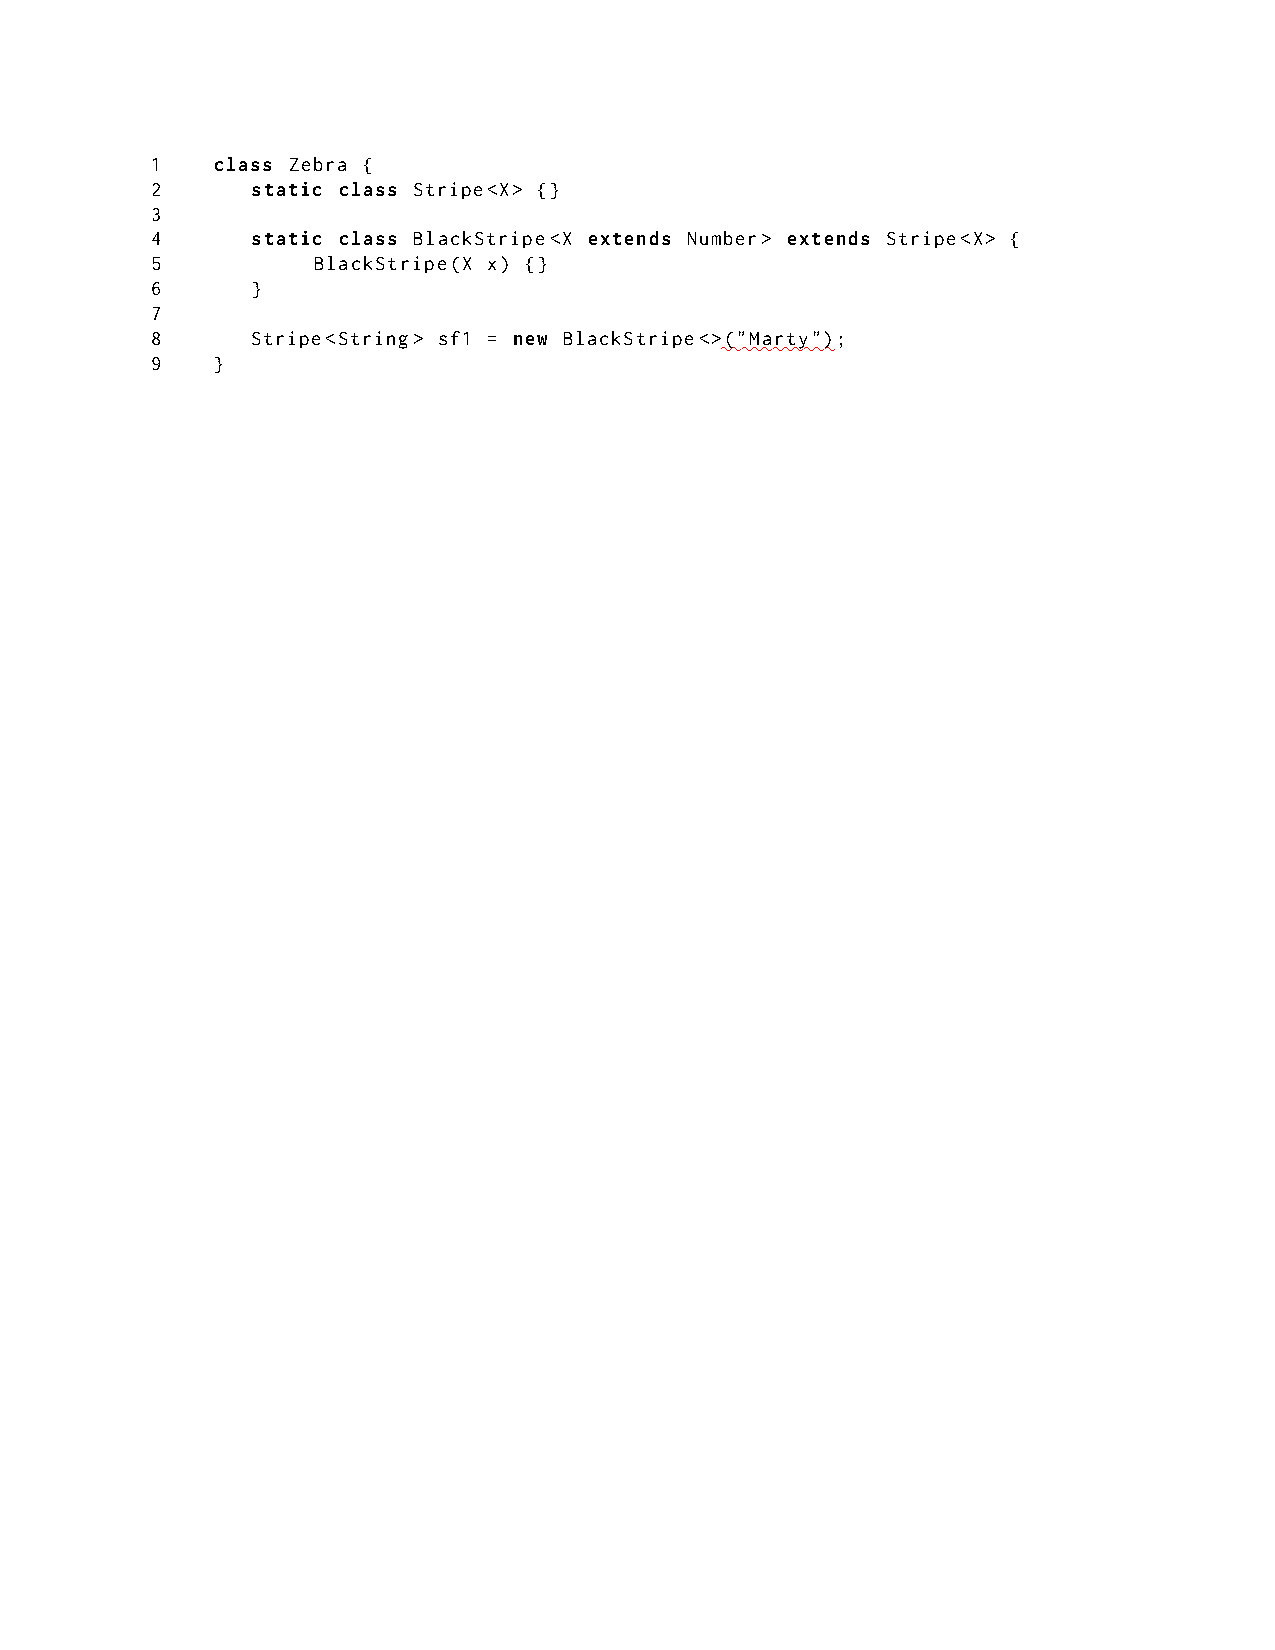
\includegraphics{zebra_wavy_crop}\label{lst:ma:traditional}}
%   \\
%   \subfloat[Explanatory visualization\label{fig:zebra:explanatory}]
%     {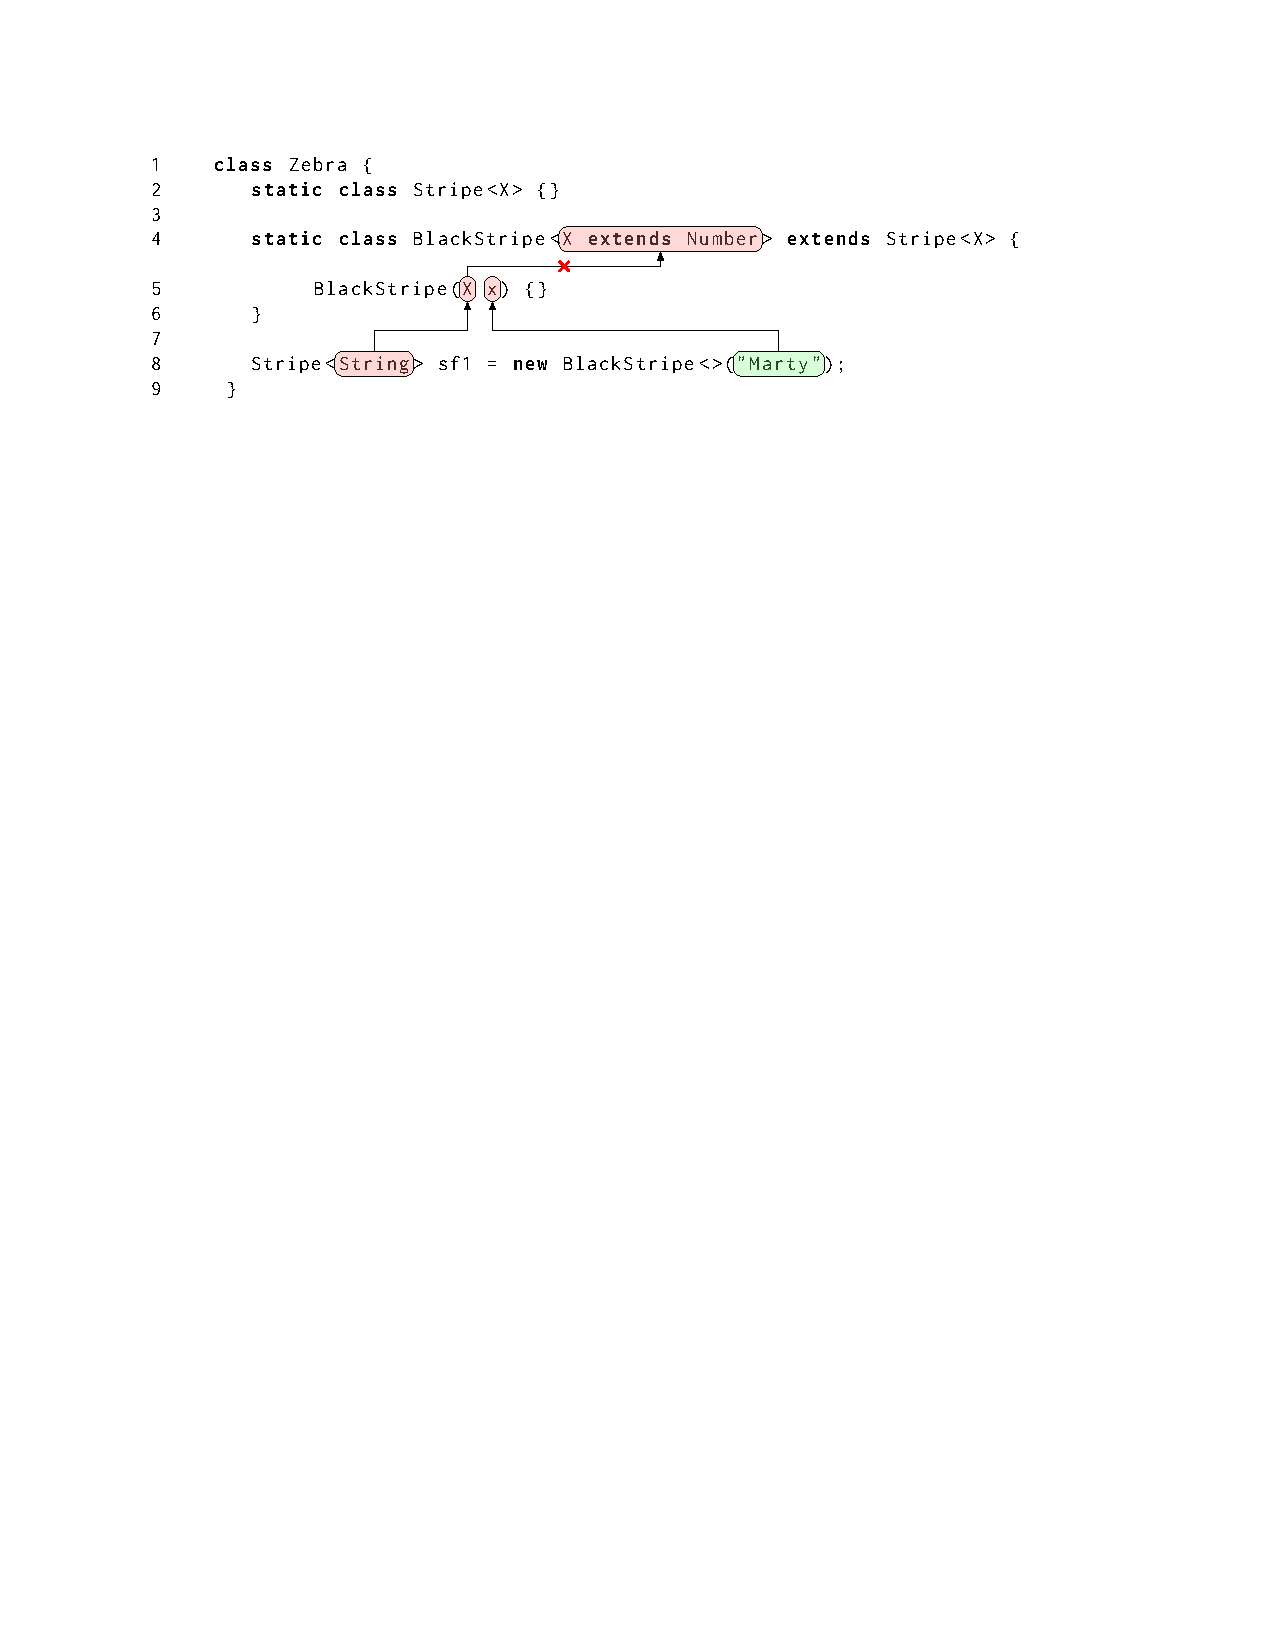
\includegraphics{zebra_explain_crop}}
%   \\
%   \subfloat[Zebra Error\label{fig:zebra:text}]{\usebox{\zebralisting}}

%   \caption{Zebra\label{fig:zebra}}
% \end{figure*}
% ==================

The purpose of this phase was to evaluate whether our explanatory visualizations resulted in more correct self-explanations by developers than with baseline visualizations (RQ1), and to identify the extent to which developers adopt conventions from our visual annotations in their own explanations (RQ2).

We sequentially provided participants with six error notifications, presented as paper mockups that resembled an IDE. For the mockup, the source code of the OpenJDK file in the mockup was minimally modified using a random-noun generator to make the class and method names more pronounceable. These tasks are summarized in Table~\ref{tab:tasks}, and we presented the tasks to the participants alphabetically by Task Name. 

In the control group, participants received paper mockups. containing the baseline red wavy underline visualization, such as in Figure~\ref{fig:melon:base}. The treatment groups received paper mockups containing our explanatory visualization as in Figure~\ref{fig:melon:explanatory}. Below the source code listing, all participants received the full error message text (Figure~\ref{fig:melon:text}). In the treatment group, we provided participants with a visual annotation legend (Table~\ref{tab:viztax}), since these participants did not have prior familiarity with our visualizations. Finally, we provided participants with colored pencils and an unadorned mockup of the IDE having the source code and error message text, but no annotations.

For each task, we provided participants with 30 seconds to individually examine the paper mockup. Then, we instructed participants to think-aloud and verbally explain the cause of the error. During their self-explanation, we encouraged participants to visually annotate the unadorned mockup. We gave participants two minutes for the think-aloud explanation, or allowed them to finish earlier if they were satisfied with their explanation for the task. The investigators were not allowed to correct the participants when they gave incorrect explanations, nor give any hints about the error notification. However, we permitted the investigators to ask clarifying questions (e.g., ``Could you explain that in more detail?'' or ``I didn't hear you. Could you repeat that?''). At the end of each explanation, participants indicated whether or not they had previously encountered this error message, which they categorized as Yes, No, or Unsure.

\subsubsection{Cognitive Dimensions Survey}
\label{subsec:cogdim}

To evaluate the aspects of visualizations that developers find useful in self-explanation (RQ3), participants completed a Cognitive Dimensions of Notations questionnaire (CD)~\cite{Green1996}, which we simplified for error message notifications. We chose this evaluation instrument over other usability instruments because the analysis is usable by non-specialists in HCI (in contrast with Nielson and Molich's heuristic evaluation~\cite{Nielsen1990}), because it uses terms that are recognizable to non-specialists, is quick to apply, and can be used in an early design phase.

The full CD defines 14 dimensions, but not all of these are applicable to our design. Since our visualizations are currently non-interactive, we eliminated all dimensions that assessed interactivity or were otherwise immaterial to our study, among them, viscosity, premature commitment, and progressive evaluation. This left four dimensions:

\begin{description}
\item[\textit{Consistency}]\hfill\\ similar semantics are expressed in similar syntactic forms
\item[\textit{Hidden dependencies}]\hfill\\ important links between entities are not visible
\item[\textit{Hard mental operations}]\hfill\\ high demand on cognitive resources
\item[\textit{Role expressiveness}]\hfill\\ the purpose of a component is readily inferred
\end{description}

A description of each dimension was presented to the participants, along with a 5-point interval scale indicating the degree to which their visualizations satisfied the dimension, which we worded so that higher scores are better. We gave participants 5 minutes to complete the questionnaire.

\subsubsection{Break} We gave participants a 5 minute break between the first and second phase of the study. In part, this was due to the lengthy duration, but also to minimize short-term memory interference between the two parts of the experiment.

\subsubsection{Phase 2: Recall Phase}

\begin{figure}[!t]
  \centering  
  \subfloat[Command prompt.\label{fig:progenv:cmd}]{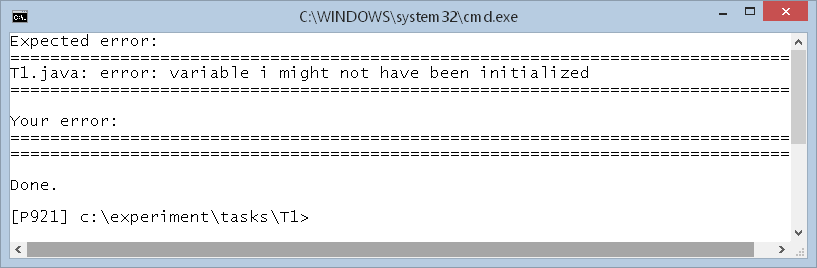
\includegraphics[width=\columnwidth]{cmd2.png}}\\
  \subfloat[Minimal text editor.\label{fig:progenv:text}]{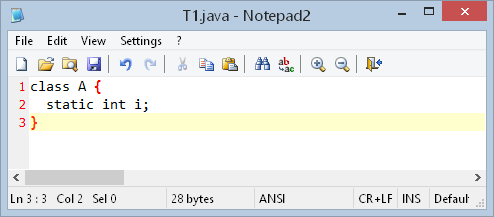
\includegraphics[width=\columnwidth]{figures/notepad22.png}}  
  \caption{We presented participants with a command prompt in which they had the \texttt{compile} command available to them. The limited interaction modality forces participants to rely solely on their own memory to successfully complete the task.\label{fig:progenv}}
\end{figure}

The purpose of this phase was to determine whether better self-explanations enable developers to better construct mental models of error notifications (RQ4). To evaluate this hypothesis, we asked participants to write source code listings on a computer from scratch in order to \textit{generate} a provided compile error. 

Participants did so through the interface shown in Figure~\ref{fig:progenv}. We gave the participants a command prompt (Figure~\ref{fig:progenv:cmd}) supporting a single command, \texttt{compile}. This command printed to the console the expected error for the task, as well as the error that their source file produced. In addition, participants entered their source code into a minimal text editor (Figure\ref{fig:progenv:text}). We chose a minimal text editor to force all participants to recall code entirely from memory, without assistive features like auto-completion. For example, in Figure~\ref{fig:progenv}, the participant has been asked to write a source listing that generates the error \texttt{variable i might not have been initialized}. However, the source listing as currently written compiles without error.

Participants used this interface to complete a total of six tasks, and they had \textit{previously explained} all of these tasks in the Self-Explanation Phase of the experiment. The tasks from this phase are also from Table~\ref{tab:tasks}, but to avoid serial recall we presented the tasks in Task Order, rather than alphabetically by Task Name. Thus, participants had to successfully \textit{recall} their explanations from the Explanation Phase of the experiment and apply their understanding to this phase of the experiment. We allowed participants an unlimited number of compilation attempts, but restricted the time for each task to 5 minutes. Participants moved on to the next task either when they had successfully replicated the error message, which we term \textit{recall correctness}, or when their time had expired.

The unusual experimental technique in this phase is not without theoretical justification. In 1977, Shneiderman conducted an experiment in which he used memorization/recall tasks as a basis for judging programmer comprehension~\cite{Shneiderman1977}. Specifically, one component of his experiment involved non-programmers and programmers memorizing a proper \texttt{FORTRAN} program printed on paper through a line printer. He also printed a second program, whose lines were shuffled. He found that non-programmers had similar performance in recall with both the proper and shuffled versions of the program, but that programmers had significantly better recall on the proper version of the program. Through the development of his cognitive syntantic/semantic model, 
he suggests that ``performance on a recall task would be a good measure of program comprehension'' because such a task cannot be accomplished by rote memorization, and instead requires ``recognizing meaningful program structures enabling them to recode the syntax of the program into a higher level internal semantic structure''~\cite{Shneiderman1977}.

Thus, participants need to have constructed a correct mental model of the error notification through self-explanation in order to successfully complete the task in this phase of the experiment.

\section{Results}

% The participant in (a) incorrectly identifies that the variable \texttt{i} must be initialized in the declaration. This in turn leads to a downstream breakdown in that \texttt{final} variables cannot be initialized more than once. The participant in (b) explains how the variable is only sometimes initialized.

\subsection{RQ1: Visualizations Lead to More Correct Explanations}
\label{subsec:result:explanation}

\begin{figure}[!t]
\centering
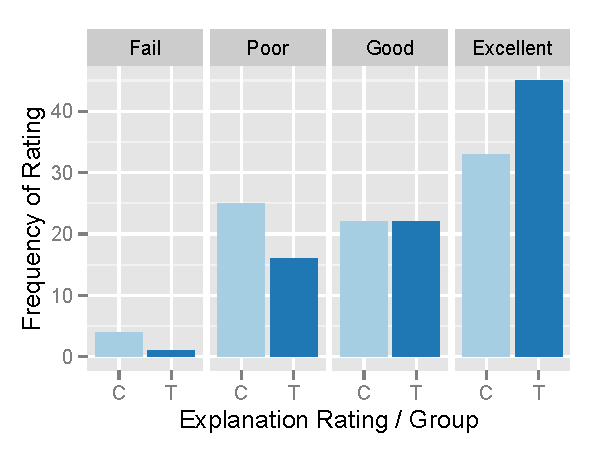
\includegraphics[width=\linewidth]{ratingbygroup}
\caption{Explanation rating by group. The treatment group (T) provided significantly higher rated explanations than the control group (C).\label{fig:ratingbygroup}}
\end{figure}

Our hypothesis was that having visual explanations for compiler notifications would yield more correct explanations by participants. To validate this hypothesis, we conducted an inter-rater reliability exercise in which the first and second authors independently rated the participants' explanations, without consideration of group. The first author assigned ratings using both the recorded verbal explanations of the participant as well as their paper markings. The second author assigned ratings using only the paper markings. This was a deliberate design decision to ascertain the extent to which visual markings alone can be used to infer the correctness of an explanation.

We assigned ratings to each of the 168 tasks on a Likert-type scale from 1--4, labeled Fail, Poor, Good, and Excellent, respectively. For each task, we developed a rubric for what constituted a correct explanation and noted common misconceptions. Cohen's Kappa (squared weights), found moderate agreement between the raters ($n = 168$, $\kappa = 0.58$, 95\% CI: $[0.46,0.68]$). Furthermore, a paired Wilcoxon Signed-Rank Test did not identify the differences between the two raters as being significant ($n_1 = n_2 = 168, S = 200, p = .21$), Thus, the data suggest that visual annotations capture the correctness of the full explanation adequately. No attempts were made to reconcile disagreement. In subsequent analysis, we use the explanation ratings from the verbal and written rater. Because this rater had access to more information from which to assign a rating, these ratings are likely to be more accurate than ratings assigned from written markings alone.

The distribution between the two groups, binned by rating, is shown in Figure~\ref{fig:ratingbygroup}. Between the control and treatment groups, a Wilcoxon Rank-Sum Test confirms that participants gave significantly better explanations in the treatment group ($n_1 = n_2 = 84, Z = 2.23, p = .026)$. A potential confound is that participants are simply providing better explanations in the treatment group because more of them had previously encountered the error messages, but a Pearson Chi-squared Test did not identify a significant difference between the groups ($n = 168$, $df = 2$, $\chi^2 = 3.37$, $p = .19$).

\subsection{RQ2: Availability of Explanatory Visual Annotations Promotes More Frequent Use of Annotations During Self-Explanation}


\begin{figure}[!t]
\centering
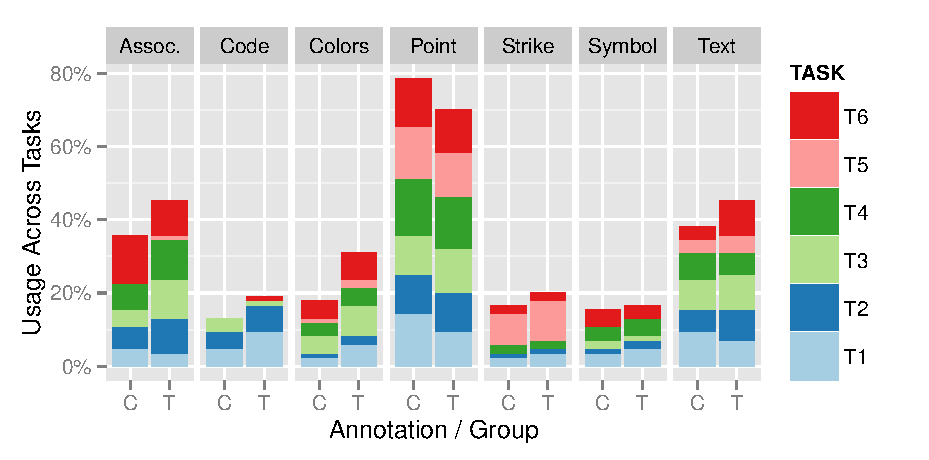
\includegraphics[width=\columnwidth]{annotation_by_group}
\caption{Annotations by group, filled with usage across tasks. The distribution of annotations used by the control (C) and treatment groups (T) were not identified as being significantly different, but the treatment group used annotations significantly more often.}\label{fig:annotationbygroup}
\end{figure}

\begin{table}[!t]
\caption{Number of Features by Task and Group\label{tab:features}}
\centering
\begin{tabular}{lrcrc}
\toprule
& \multicolumn{4}{c}{Number of Features}\\ \cmidrule(lr){2-5}
 & \multicolumn{2}{c}{Control}& \multicolumn{2}{c}{Treatment}\\
 \cmidrule(lr){2-3} \cmidrule(lr){4-5}
 Task & Median & Dist & Median & Dist\\ 
\midrule
T1 & 
2 &
\definecolor{sparkspikecolor}{named}{darkgray}
\begin{sparkline}{4}
\sparkspike .083 .4
\sparkspike .25 1
\sparkspike .417 .6
\sparkspike .583 .2
\sparkspike .75 .2
\end{sparkline}
&
3 &
\definecolor{sparkspikecolor}{named}{olive}
\begin{sparkline}{4}
\sparkspike .083 .2
\sparkspike .25 .4
\sparkspike .417 0.6
\sparkspike .583 0.4
\sparkspike .75 0.01
\end{sparkline}
\\

T2 &
2 & \definecolor{sparkspikecolor}{named}{darkgray}
\begin{sparkline}{4}
\sparkspike .083 .2
\sparkspike .25 1
\sparkspike .417 .6
\sparkspike .583 .01
\sparkspike .75 .01
\end{sparkline}
&
2 & \definecolor{sparkspikecolor}{named}{olive}
\begin{sparkline}{4}
\sparkspike .083 .2
\sparkspike .25 .8
\sparkspike .417 .4
\sparkspike .583 .2
\sparkspike .75 0.01
\end{sparkline}
\\


T3 &
2 & 
\definecolor{sparkspikecolor}{named}{darkgray}
\begin{sparkline}{4}
\sparkspike .083 .17
\sparkspike .25 1
\sparkspike .417 .17
\sparkspike .583 .17
\sparkspike .75 0.01
\end{sparkline}
&
2 &
\definecolor{sparkspikecolor}{named}{olive}
\begin{sparkline}{4}
\sparkspike .083 .17
\sparkspike .25 .83
\sparkspike .417 .33
\sparkspike .583 .33
\sparkspike .75 .01
\end{sparkline}
\\

T4 &
2 & \definecolor{sparkspikecolor}{named}{darkgray}
\begin{sparkline}{4}
\sparkspike .083 .5
\sparkspike .25 .83
\sparkspike .417 0.33
\sparkspike .583 0.5
\sparkspike .75 0.01
\end{sparkline}
&
3 & \definecolor{sparkspikecolor}{named}{olive}
\begin{sparkline}{4}
\sparkspike .083 .33
\sparkspike .25 .33
\sparkspike .417 1
\sparkspike .583 .33
\sparkspike .75 .01
\end{sparkline}
\\

T5 &
1 & \definecolor{sparkspikecolor}{named}{darkgray}
\begin{sparkline}{4}
\sparkspike .083 1
\sparkspike .25 .67
\sparkspike .417 0.17
\sparkspike .583 0.17
\sparkspike .75 0.01
\end{sparkline}
&
2 & \definecolor{sparkspikecolor}{named}{olive}
\begin{sparkline}{4}
\sparkspike .083 .33
\sparkspike .25 .83
\sparkspike .417 .33
\sparkspike .583 .17
\sparkspike .75 .01
\end{sparkline}
\\

T6 &
3 & \definecolor{sparkspikecolor}{named}{darkgray}
\begin{sparkline}{4}
\sparkspike .083 .33
\sparkspike .25 .33
\sparkspike .417 1
\sparkspike .583 0.17
\sparkspike .75 0.01
\end{sparkline}
&
3 & \definecolor{sparkspikecolor}{named}{olive}
\begin{sparkline}{4}
\sparkspike .083 .01
\sparkspike .25 .5
\sparkspike .417 .83
\sparkspike .583 0.33
\sparkspike .75 .01
\end{sparkline}\\
\bottomrule
\end{tabular}
\end{table}

Our hypothesis was that both the control group and treatment group would adopt similar annotations when developers explained error messages, if these annotations were grounded in conventions that developers found to be intuition.

Consider for a moment the visualizations drawn by two participants in our study, shown in Figure~\ref{fig:partmelon}. In Figure~\ref{fig:partmelon:control}, the control group participant receives a score of Fail, because he incorrectly self-explains that the problem must be due to not initializing the variable at its point of declaration. He then either ignores the conditional statement in which the constant value is re-assigned, or fails to notice that the variable is declared as \texttt{final}. In Figure~\ref{fig:partmelon:treatment}, the participant, aided by the explanatory visualization, correctly self-explains that the problem is actually in the conditional statement, and provides explanatory code to demonstrate a case in which the variable remains uninitialized. In addition, the treatment participant uses more annotations, such as colors, points, and associations, in his explanation than the control group participant.

Table~\ref{tab:features} summarizes the number of annotation types used for each task, partitioned by control and treatment groups. Using a Wilcoxon Rank-Sum Test, we find that there the treatment group using significantly more visual annotation types in their explanations than the control group ($n_1 = n_2 = 84$, $Z = 2.15$, $p = .032$).

One concern is that participants in the treatment group used these annotations simply because they were readibly \textit{available}, and not because they were \textit{useful} to their explanations. Figure~\ref{fig:annotationbygroup} shows the distribution of the annotations by group. The bars are filled with the usage of that annotation by task to indicate how a particular annotation is distributed among the tasks. A Pearson Chi-squared Test was unable to identify any significant differences in the \emph{distribution} of these annotation types ($n = 389$, $\chi^2 = 4.20$, $df = 5$, $p = .65$). Figure~\ref{fig:annotationbygroup} also shows that the control group used the point annotation more than the treatment group, but this different was not found to be significant ($n = 168$, $df = 1$, $\chi^2 = 1.53$, $p = .22$).

In addition, none of the participants in the treatment group used our invented code coverage annotation, nor did this annotation appear directly in our pilot study. This suggests that explanatory visualizations promote usage in developers, and that participants are using these annotations only when they find them to be useful in self-explanation.

Thus, participants in both groups use and apply the annotations found in our explanatory visualizations, despite the fact that we did not give the control group knowledge of our visualizations. This indicates that these annotations are intuitive and useful for participants. Moreover, the presence of explanatory visualizations promotes their usage during self-explanation in participants.

\begin{figure}[!t]
  \centering
  \subfloat[\label{fig:partmelon:control}]
    { 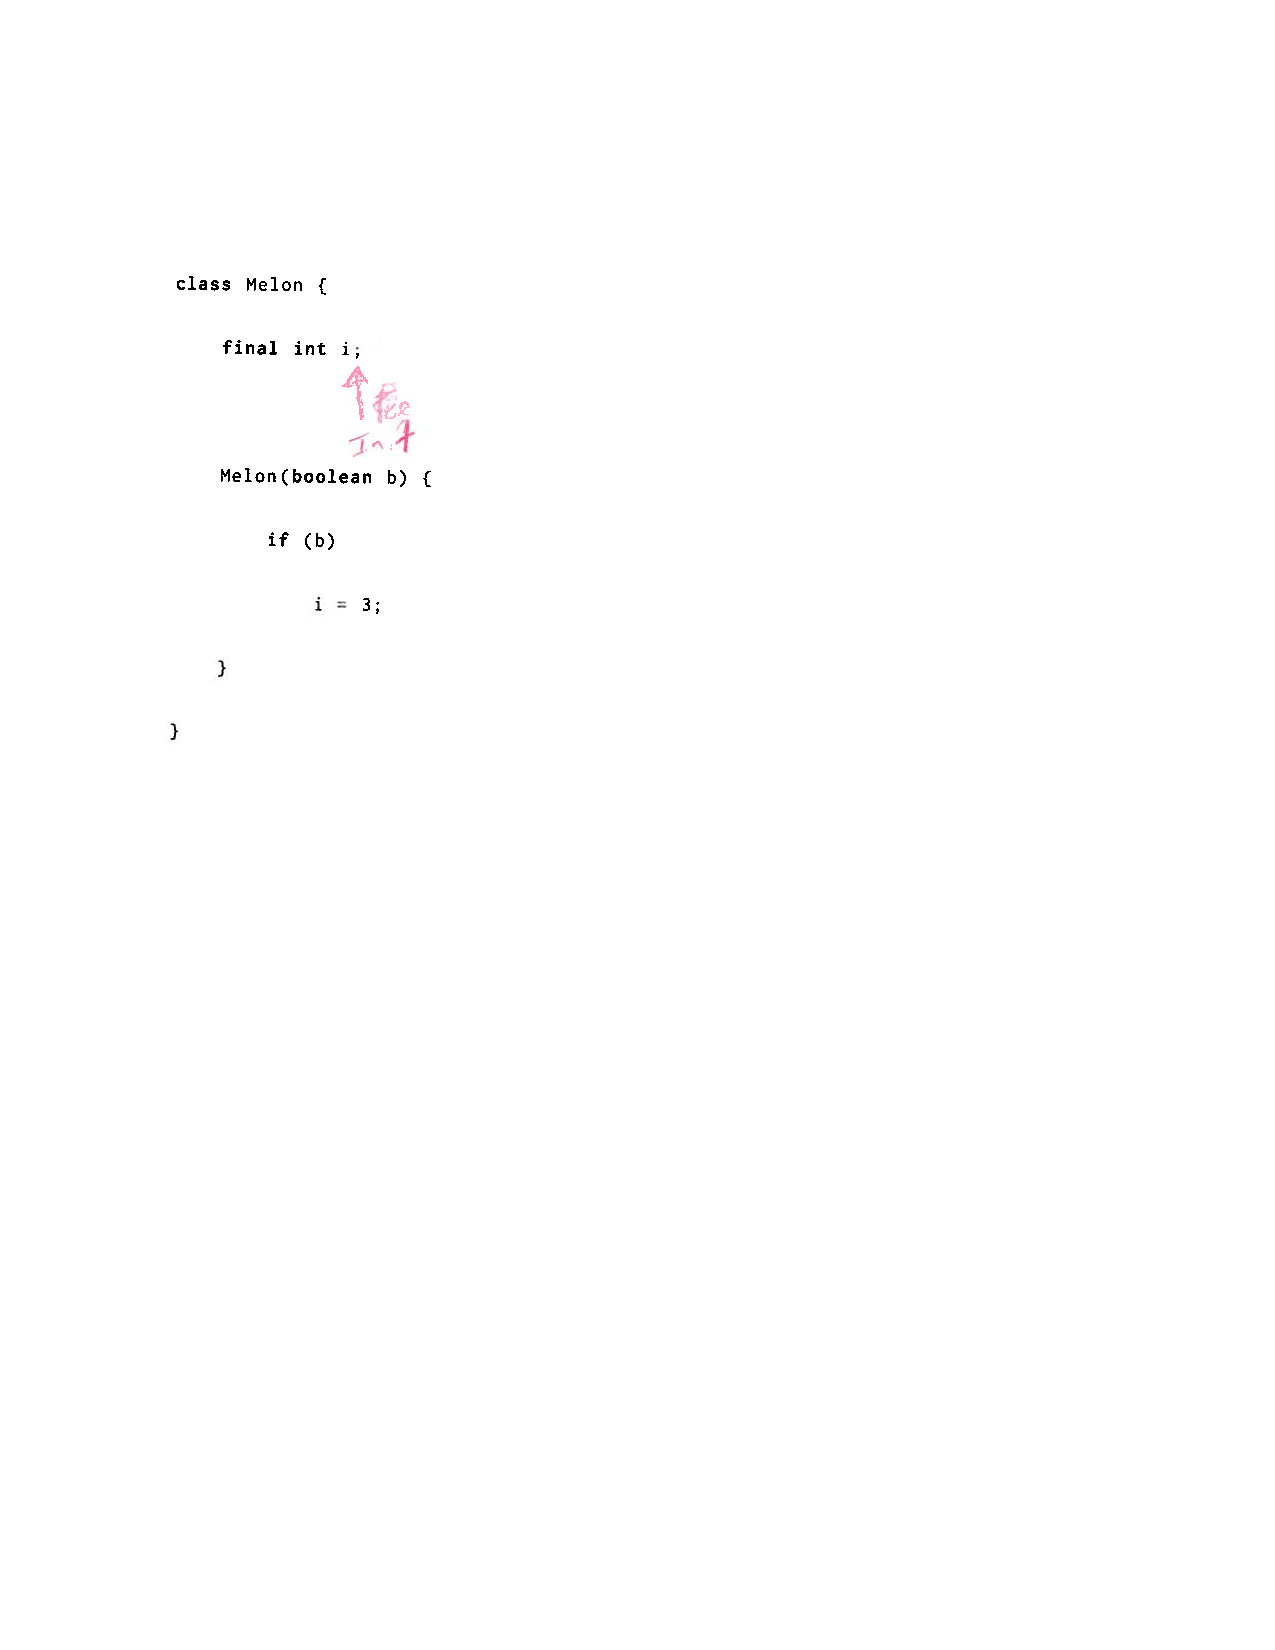
\includegraphics[height=2.5in]{P658_melon} }
  \subfloat[\label{fig:partmelon:treatment}]
    {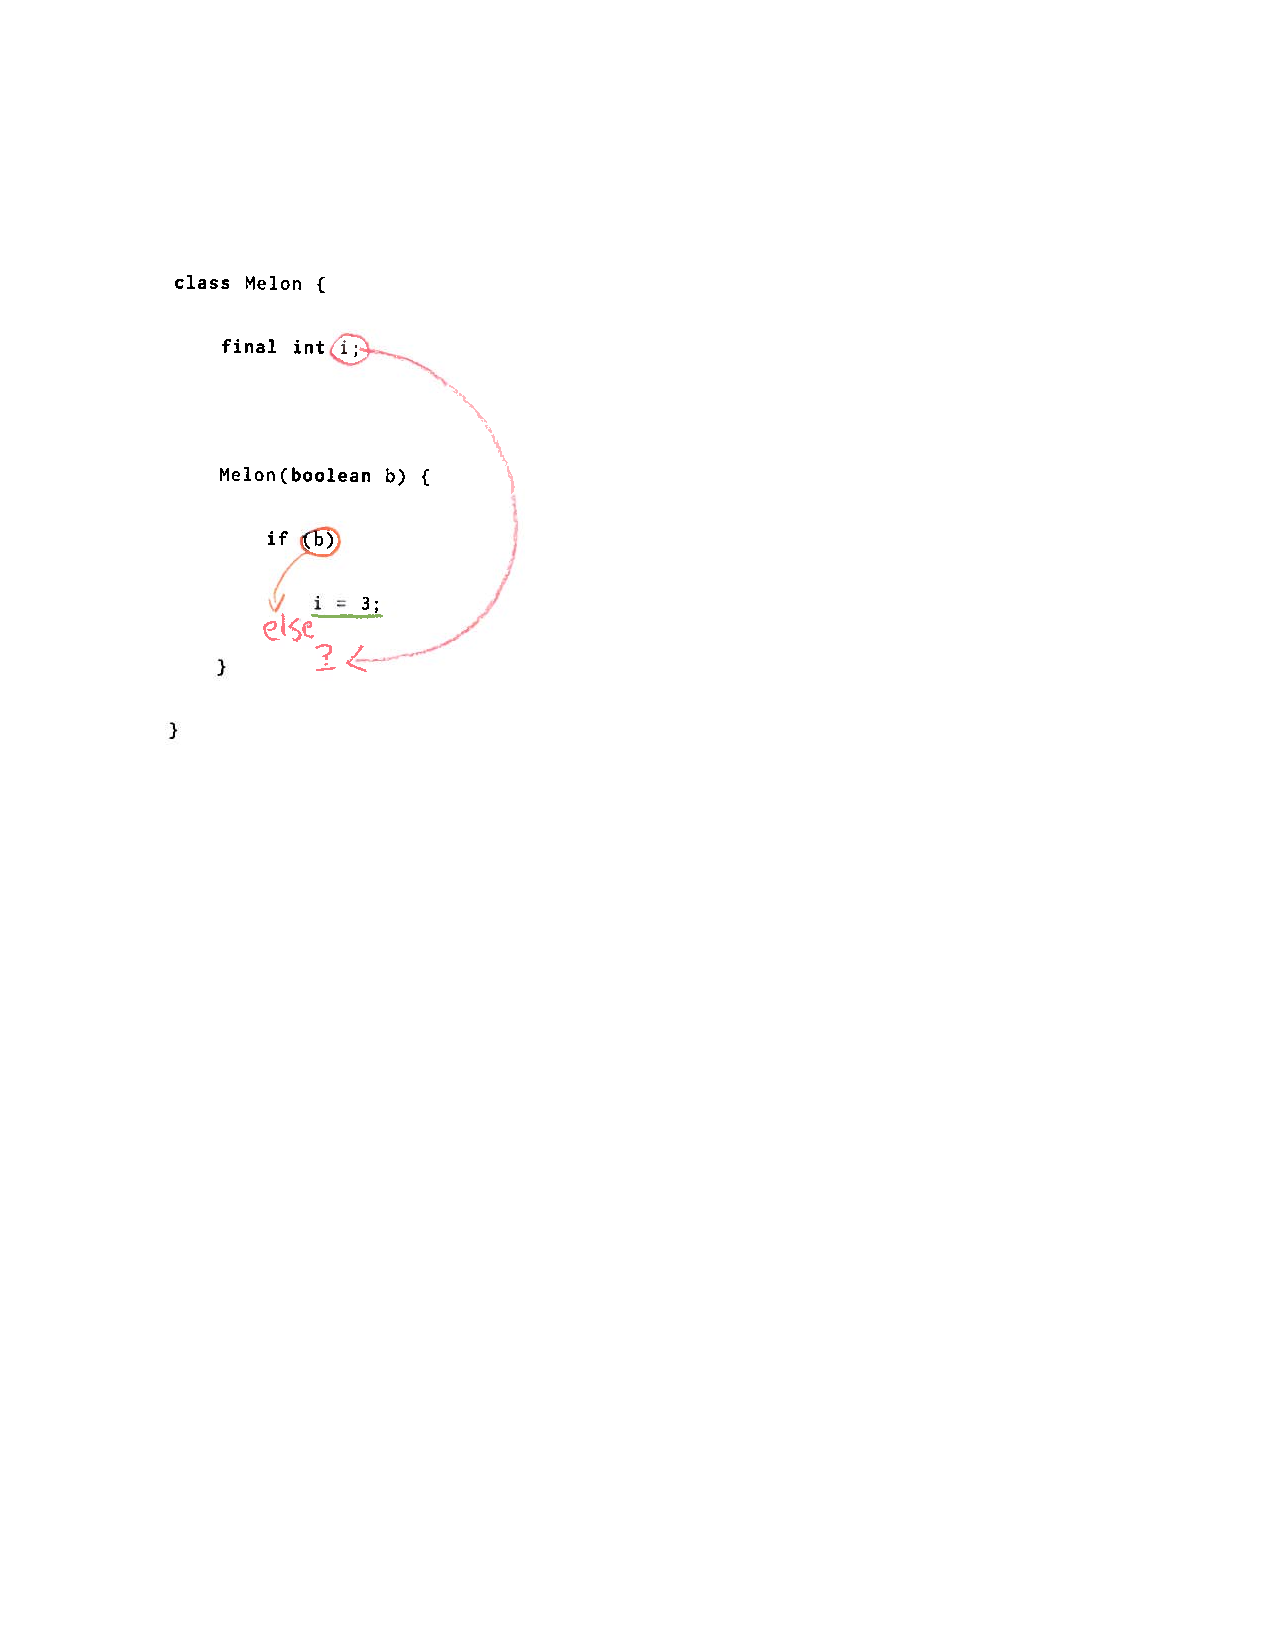
\includegraphics[height=2.5in]{P469_melon}}
  \caption{A contrast between visual explanations offered by (a) control group participant with explanation rating of Fail, and (b) treatment group participant with explanation rating of Excellent. \label{fig:partmelon}}
\end{figure}


\subsection{RQ3: Explanatory Visualizations Reveal Hidden Dependencies}

% TODO: Column for number of responses?
\begin{table}[!t]
\caption{Cognitive Dimensions Questionnaire Responses\label{tab:cogdim}}
\centering
% Some packages, such as MDW tools, offer better commands for making tables
% than the plain LaTeX2e tabular which is unsolved here.
\begin{tabular}{lrcrcr}
\toprule
 & \multicolumn{2}{c}{Control}& \multicolumn{2}{c}{Treatment}\\
 \cmidrule(lr){2-3} \cmidrule(lr){4-5}
 Dimension & Median & Dist & Median & Dist & $p$\\ 
\midrule

%\textbf{Hidden Dependencies} & \textbf{Consistency} & \textbf{Hard %mental operations} & \textbf{Role Expressiveness} \\
%\midrule
Hidden Dependencies\textsuperscript{*} & 
3 &
\definecolor{sparkspikecolor}{named}{darkgray}
\begin{sparkline}{4}
\sparkspike .083 .01
\sparkspike .25 .83
\sparkspike .417 .1
\sparkspike .583 .33
\sparkspike .75 .17
\end{sparkline}
&
4 &
\definecolor{sparkspikecolor}{named}{olive}
\begin{sparkline}{4}
\sparkspike .083 .01
\sparkspike .25 .17
\sparkspike .417 0.5
\sparkspike .583 0.83
\sparkspike .75 0.83
\end{sparkline}
& .008
\\

Consistency &
4 & \definecolor{sparkspikecolor}{named}{darkgray}
\begin{sparkline}{4}
\sparkspike .083 .01
\sparkspike .25 .125
\sparkspike .417 .125
\sparkspike .583 1
\sparkspike .75 0.5
\end{sparkline}
&
4 & \definecolor{sparkspikecolor}{named}{olive}
\begin{sparkline}{4}
\sparkspike .083 .01
\sparkspike .25 .01
\sparkspike .417 .25
\sparkspike .583 1
\sparkspike .75 0.5
\end{sparkline}
& .979
\\


Hard Mental Operations &
3 & 
\definecolor{sparkspikecolor}{named}{darkgray}
\begin{sparkline}{4}
\sparkspike .083 .01
\sparkspike .25 .86
\sparkspike .417 .86
\sparkspike .583 .29
\sparkspike .75 0.01
\end{sparkline}
&
2.5 &
\definecolor{sparkspikecolor}{named}{olive}
\begin{sparkline}{4}
\sparkspike .083 .01
\sparkspike .25 1
\sparkspike .417 .71
\sparkspike .583 .14
\sparkspike .75 .14
\end{sparkline}
& .821
\\

Role Expressiveness &
4 & \definecolor{sparkspikecolor}{named}{darkgray}
\begin{sparkline}{4}
\sparkspike .083 .13
\sparkspike .25 .13
\sparkspike .417 0.5
\sparkspike .583 0.88
\sparkspike .75 0.13
\end{sparkline}
&
4 & \definecolor{sparkspikecolor}{named}{olive}
\begin{sparkline}{4}
\sparkspike .083 .01
\sparkspike .25 .01
\sparkspike .417 .38
\sparkspike .583 1
\sparkspike .75 .38
\end{sparkline}
& .130
\\

\bottomrule
\end{tabular}
\end{table}

We wanted to discover which factors participants considered to be significant improvements over the baseline visualization. We had no explicit hypothesis for this research question.

Table~\ref{tab:cogdim} summarizes the results from our Cognitive Dimensions questionnaire. Median results for the hidden dimensions for control and treatment groups were 3 and 4, respectively. The distribution of responses in the two groups were significantly different ($n_1 = n_2 = 14$, $Z = -2.64$, $p = .008$). The result suggests that our explanatory visualizations reveal more of the hidden dependencies, that is, the internal reasoning process of the compiler, than the baseline visualizations.

We were unable to identify any statistically significant differences from the remaining dimensions in the questionnaire.

% \subsection{Participants Reliably Self-Assess Explanatory Correctness}

% \begin{table}[!t]
% \caption{Confidence by Previously Encountered Error Messages by Group\label{tab:confidenceencounter}}
% \centering
% \begin{tabular}{lrcrc}
% \toprule
% & \multicolumn{4}{c}{Confidence}\\
% \cmidrule(lr){2-5}
%  & \multicolumn{2}{c}{Control}& \multicolumn{2}{c}{Treatment}\\
%  \cmidrule(lr){2-3} \cmidrule(lr){4-5}
%  Encountered & Median & Dist & Median & Dist\\ 
% \midrule
% Yes & 
% 3 &
% \definecolor{sparkspikecolor}{named}{darkgray}
% \begin{sparkline}{4}
% \sparkspike .083 .01
% \sparkspike .25 .07
% \sparkspike .417 .06
% \sparkspike .583 1
% \sparkspike .75 .06
% \end{sparkline}
% &
% 3.5 &
% \definecolor{sparkspikecolor}{named}{olive}
% \begin{sparkline}{4}
% \sparkspike .083 .01
% \sparkspike .25 .01
% \sparkspike .417 0.71
% \sparkspike .583 1
% \sparkspike .75 0.5
% \end{sparkline}
% \\

% Unsure &
% 3 & \definecolor{sparkspikecolor}{named}{darkgray}
% \begin{sparkline}{4}
% \sparkspike .083 .6
% \sparkspike .25 .4
% \sparkspike .417 .6
% \sparkspike .583 1
% \sparkspike .75 .2
% \end{sparkline}
% &
% 4 & \definecolor{sparkspikecolor}{named}{olive}
% \begin{sparkline}{4}
% \sparkspike .083 .01
% \sparkspike .25 .4
% \sparkspike .417 .2
% \sparkspike .583 .6
% \sparkspike .75 0.2
% \end{sparkline}
% \\

% No &
% 4 & \definecolor{sparkspikecolor}{named}{darkgray}
% \begin{sparkline}{4}
% \sparkspike .083 .36
% \sparkspike .25 0.5
% \sparkspike .417 .57
% \sparkspike .583 .71
% \sparkspike .75 .5
% \end{sparkline}
% &
% 4 & \definecolor{sparkspikecolor}{named}{olive}
% \begin{sparkline}{4}
% \sparkspike .083 .14
% \sparkspike .25 .64
% \sparkspike .417 .86
% \sparkspike .583 1
% \sparkspike .75 0.64
% \end{sparkline}
% \\

% \bottomrule
% \end{tabular}
% \end{table}

% Our hypothesis is that participants who are more confident in their explanation would also receive higher ratings, and that participants would be more confident in the treatment group because the visual annotations are more expressive and provide more explanation.

% Table~\ref{tab:confidenceencounter} summarizes the distribution confidence for each of the participants in each group, by whether or not the participant has previous encountered a given error message. Through a Kruskal-Willis Test, we identified a significant effect in the confidence of participant explanations as a result of having encountered the error message ($\chi^2 = 11.26$, $df = 2$, $p = 0.004$). This result, by itself, is not particularly surprising. However, a significant difference remained for the control group ($\chi^2 = 8.13$, $df = 2$, $p = 0.01$), but not for the treatment group ($\chi^2 = 3.47$, $df = 2$, $p = 0.17$). One explanation for this is that in control group, past experience plays an important part in the participant's explanations because the visualization does not reveal much. In contrast, we speculate that in the treatment group this effect is in part neutralized by the additional explanatory capability of the visualization. However, we can only speculate because the statistical tests do not allow us to accept a null hypothesis. However, but Kendall's $\tau_b$ Rank Correlation Test revealed minimal association between previous encounter and confidence ($\tau_b = .19$). DO a mean rank instead.

% Using a Wilcoxon Rank-Sum Test, we were unable to identify statistically significant differences in participants in their reporting of confidence between the control and treatment groups ($n_1=n_2=84$, $Z = 0.58$, $p = 0.55$), though we know from the previous section that the treatment group has significantly higher explanation quality. 

% \begin{figure}[!t]
% \centering
% 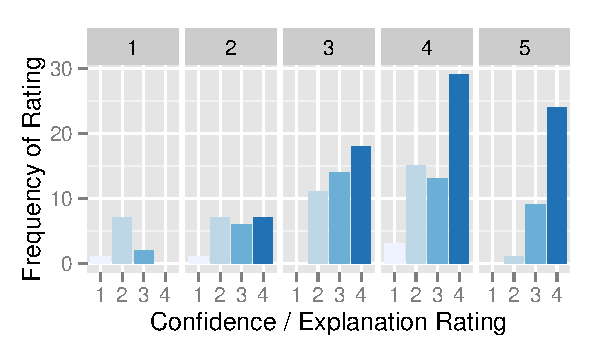
\includegraphics[width=\columnwidth]{confidence_explanation}
% \caption{Task by Explanation Rating -- we need this later, but we just broke it down by bask. also remove overlay of correctness and put this in a different figure}\label{fig:explanationbytask}
% \end{figure}

% However, just because a participant is confident in their explanation does not necessarily mean that their explanation is actually correct. This effect of confidence for each explanation rating was statistically significant ($X^2 = 19.42$, $df = 3$, $p < 0.001$). mean ranks.

% participants know when they don't know... hmmm something is broken here with this and the KSCORE

% , but Kendall's $\tau_b$ Rank Correlation Test revealed little to weak association ($\tau_b = 0.29$), and the sum of ranks did not show consistent increase with explanation rating.

\subsection{RQ4: Higher Rated Explanations Lead to Better Mental Models, and Better Recall Correctness}

\begin{figure}[!t]
\centering
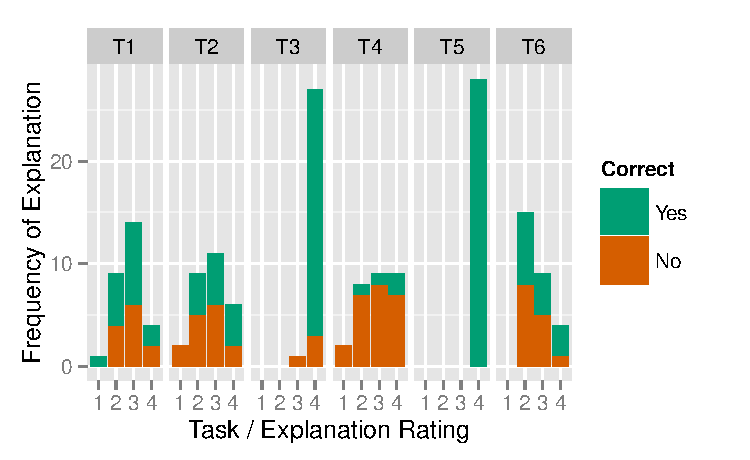
\includegraphics[width=\columnwidth]{explanation_by_task}
\caption{Task by explanation rating. Each of the six tasks are broken by explanation rating (1 = Fail, 2 = Poor, 3 = Good, 4 = Excellent) from the first phase of the experiment. For each explanation rating, the frequency of correct and incorrect recall tasks from the second phase of the experiment is indicated by filling in the bars. Higher rated explanations lead to significantly better recall correctness.}\label{fig:explanationbytask}
\end{figure}

Figure~\ref{fig:explanationbytask} illustrates the explanation rating for each task, the frequency of the explanation for each rating within the task, and the recall correctness. Remember from Section~\ref{subsec:result:explanation} that explanation correctness by group was significant, in that the treatment group had higher explanation ratings. Thus, our expectation was that these higher rated explanations would translate to better correctness scores during the recall phase of the experiment.

A Kruskal-Wallis Test revealed a significant difference between performance on explanation correct and performance on recall correctness ($\chi^2 = 29.39$, $df = 3$, $p < .001$), and the mean ranks indicate that recall correctness generally increases with explanation correctness ($u_1 = 51.8$, $u_2 = 69.8$, $u_3 = 69.3$, $u_4 = 102.8$). This confirms that explanation is valuable for improving correctness in the recall task, but two potentially problematic issues arise.

In Figure~\ref{fig:explanationbytask}, we observe that recall task T5 (redundant modifier) has both perfect recall correctness and uniformly excellent explanation rating, which we postulate is attributable to this being trivial problem. Our first concern is that this task is artificially inflating the influence of the explanation task to recall correctness. For example, we visually identify that T4 has some participants who have an excellent explanation rating, but even excellent explanations translate to limited success during the recall phase of the experiment. As a result of this skepticism, we re-ran the analysis after removing T5. We found that the result is still significant ($\chi^2 = 12.33$, $df = 3$, $p = 0.006$), and the general trend remains ($u_1 = 49.0$, $u_2 = 64.0$, $u_3 = 63.6$, $u_4 = 84.0$).

% Of course, one might also argue that T3 should also be removed on similar ground, but this decision is more contentious, since variation exists in both explanation rating and correctness for this task. But in the interest of full disclosure, removing T3 and T5 removes the significance ($\chi^2 = 1.30$, $df = 3$, $p = 0.73$), but not the trend ($u_1 = 44.2$, $u_2 = 56.21$, $u_3 = 56.44$, $u_4 = 59.78$). 

However, a second problematic issue remains --- if the treatment group gives higher rated explanations, then we would expect that they have greater correctness in recall. However, we were unable to identify this as being significant ($n_1 = n_2 = 84$, $Z = 1.09$, $p = 0.27$).

We conclude that explanation ratings improve recall correctness, though with some reservations.

% \subsection{Removing Participant Experience as a Confound}

% We had a concern that all we were really measuring was the experience of the participant, and that the explanation task was immaterial to the recall correctness. In the case of experience with Java, this particular question was useless -- 19 participants (67.9\%) reported that they were knowledgeable about Java and the remaining 9 participants (32.1\%) reported that they very knowledgeable about Java. With respect to general programmer ability, Kruskal-Wallis Test was unable to identify any significant differences between ability and either explanation rating ($\chi^2 - 3.02$, $df = 2$, $p = 0.22$) or recall correctness ($\chi^2 = 2.04$, $df = 2$, $0.36$). A logistic fit failed of industry experience also failed to identify any significance with either explanation rating ($R^2 = 0.0005$, $\chi^2 = 0.199$, $df = 1$, $p = 0.655$) or recall correctness ($R^2 = 0.001$, $\chi^2 = 0.252$, $df = 1$, $p = 0.616$). Thus, we are unable to identify any self-reported experience measures that significantly influenced the performance of the participants. Of course, we recognize that one possibility is that undergraduate students are poor assessors of their own abilities.

\section{Threats to Validity}
\label{sec:threats}

% There are several threats of validity, some of which are endemic to the use of paper mockups. Because the mockups were not automatically generated, the possibility exists that the visualizations are presented in a way that could not feasibly be generated by an actual compiler. That is, our visualization system assumes a priori the existence of a compiler that can provide it with the necessary data structure.

% External validity
In real code bases, developers have to explain error messages in functional code intertwined with erroneous code, and across multiple source files. Our tasks contained only the code directly pertinent to generating the error, and within a single source file. We don't yet know if explanatory visualizations will be equally beneficial and scale to more realistic contexts.

We applied a set of visualizations to only six hand-selected tasks that could fit on a single screen. As such, it remains to be seen whether visual annotations can be effectively applied to the broader set of error messages, including those in languages other than Java. Thus, we cannot and do not claim that these annotations are comprehensive.

% Ecological validity: Methods, materials and setting of the study must approximate the real-world that is being examined.
We think there exists a construct validity problem in that explanation ratings were significantly better in the treatment group, but this performance did not translate to better recall correctness. We postulate that this situation occurred because it was possible for developers to successfully explain the task, yet still have gaps in their mental model that preclude them from successfully completing the task. In addition, we observed that some participants had significant difficulties with syntax, and in some cases even introduced secondary compiler errors not related to the recall task in the process.

% A construct validity
Furthermore, the act of performing a think-aloud can enhance self-explanation, and in turn, the construction of mental models for notifications. This process was necessary in order to evaluate participant explanations, but in doing so, we may have unintentionally enhanced the performance of the control group in their recall tasks. A second issue is that participants were already familiar with the baseline visualizations, but had no prior experience or any training with our explanatory visualizations. This may explain why we found no statistical difference in hard mental operations: the potential cognitive benefit of our visual annotations was counterbalanced by having to understand an unfamiliar visualization.

% We incorrectly assumed that students understood the syntax of generics before participants in the experiment. However, T6 shows that participants were largely unable to complete this task, even when they had high explanation ratings. (Figure~\ref{fig:explanationbytask}).

\section{Related Work}

\textit{Self-explanation.} Lim and colleagues demonstrate that explanations describing why a system behaves a certain way results in better understanding and stronger feelings of trust~\cite{Lim2009}. We were also inspired by the work of Ainsworth and Th~Loizou, who showed that the use of diagrams promote the self-explanation effect significantly more than text~\cite{Ainsworth2003}.

\textit{Improving error notification comprehension.} Jeffrey created a tool called \textit{Merr} that overrides the error handler of the LR parser generator of a compiler to automatically provide more useful syntax error messages~\cite{Jeffery2003}, and Kantorowitz and Laor likewise propose modifications to the parser generator~\cite{Kantorowitz1986}. While these tools apply to text error messages, it illustrates that tools can improve error messages when they can interact with compiler internals. However, Nienaltowski and colleagues found that even detailed messages do not necessarily simplify understanding of error messages~\cite{Nienaltowski2008}. 

Hartmann and colleagues introduce a social recommendation system that presents examples of how other developers understand and correct errors~\cite{Hartmann2010}. In contrast, our approach argues that the compiler itself can offer its own reasoning process to aid developer comprehension. Other approaches attempt to provide better diagnostics or reduce false positives in compiler errors~\cite{Boustani2011,Campbell2014}. We expect that our visualizations can leverage such improvements in compiler technology. 


% http://dl.acm.org/citation.cfm?id=1879229
% guidelines
% http://faculty.washington.edu/ajko/papers/Lee2011Gidget.pdf
% http://dl.acm.org/citation.cfm?id=1984699 -- transparent compiler
% http://www.lucas.ezzoterik.com/papers/LWS08.
% http://www.sciencedirect.com/science/article/pii/S0167642312000469
% http://lampwww.epfl.ch/~rompf/pldi2014.pdf
% http://www.microsoft.com/en-us/download/details.aspx?id=27744

% AnimPascal

\section{Future Work}

We suggest several potential research directions. One direction is the feasibility challenge of developing algorithms and techniques for recording compiler analysis traces such that they can be exposed to visualization systems. We know that compilers generate a significant amount of information during the compilation process, but it remains an open question as to what information is pertinent to aiding developer comprehension, and how to represent this information in a way that is usable by visualization systems. One approach to demonstrate this feasibility may be to modify an implementation such as MiniJava, a useful but restricted subset of the Java language~\cite{Roberts2001}.

Another research direction is empirical: we need to determine the extent to which visualizations can be applied to error notifications, given that some annotations appear to be more suitable than others for certain notifications. A systematic investigation into categorizing these error messages, such as through taxonomy construction, may offer researchers insights into this design space.

% Such a taxonomy may also be needed to understand the types of visualizations, the composability of these them, as well as their cognitive fit --- or an Moody states, we need to establish the ``physics''of these notations~\cite{Moody2009a}. Our current work has admittely sidestepped this issue through an informal pilot study, but these issue will need to be addressed to make progress in this research area.

% Yet another research direction is in discovery approaches to presenting the visualizations algorithmically. We cannot expect tool designers to hand-craft algorithms for every individual error notification that a compiler can present. The use of domain-specific languages, as well as the invention of algorithms that can automatically place, route, and compose visualizations, will assist in this area.

\section{Conclusion}

Our work in this paper demonstrates the potential for facilitating developer self-explanations when opaque compiler reasoning processes are made available for visualization. Through error notifications, we demonstrated when such visualizations align with developer expectations, developers better comprehend error notifications, use these visualizations more often in their own self-explanations, and construct better mental models of error notifications. We think the diagrammatic techniques developers use to explain problems to other developers and to themselves can serve as an effective foundation for how IDEs should visually communicate to developers.

\section*{Acknowledgment}

This material is based upon work supported by the National Science Foundation under Grant No. 1217700. We thank the Software Engineering group at ABB Corporate Research for their funding and support.

% our system was new, they had never seen it before. if they were trained they might find it more valuable. that is promising.

% squiggly lines... why weren't they consistent? we think this is because the notation is the same but the meaning changes. in constrast, our system has different symbols for meanings, but you also have more symbols to learn.

% why explains correctness? not a tutorial system. when concepts are fuzzy, can help avoid misconceptions

% Could generalize to static analysis tools as well, which could improve usefullness and unified, allowing for better transfer of knowledge between programming languages.

% Developers didn't seem to actually read the error message, but rather just looked at the squiggly lines.  (Further motivating our approach)

% ``Trained to ignore error message'', learned helplessness from bad error messages.

% An example of a floating figure using the graphicx package.
% Note that \label must occur AFTER (or within) \caption.
% For figures, \caption should occur after the \includegraphics.
% Note that IEEEtran v1.7 and later has special internal code that
% is designed to preserve the operation of \label within \caption
% even when the captionsoff option is in effect. However, because
% of issues like this, it may be the safest practice to put all your
% \label just after \caption rather than within \caption{}.
%
% Reminder: the "draftcls" or "draftclsnofoot", not "draft", class
% option should be used if it is desired that the figures are to be
% displayed while in draft mode.
%
%\begin{figure}[!t]
%\centering
%\includegraphics[width=2.5in]{myfigure}
% where an .eps filename suffix will be assumed under latex, 
% and a .pdf suffix will be assumed for pdflatex; or what has been declared
% via \DeclareGraphicsExtensions.
%\caption{Simulation Results}
%\label{fig_sim}
%\end{figure}

% Note that IEEE typically puts floats only at the top, even when this
% results in a large percentage of a column being occupied by floats.


% An example of a double column floating figure using two subfigures.
% (The subfig.sty package must be loaded for this to work.)
% The subfigure \label commands are set within each subfloat command, the
% \label for the overall figure must come after \caption.
% \hfil must be used as a separator to get equal spacing.
% The subfigure.sty package works much the same way, except \subfigure is
% used instead of \subfloat.
%
%\begin{figure*}[!t]
%\centerline{\subfloat[Case I]\includegraphics[width=2.5in]{subfigcase1}%
%\label{fig_first_case}}
%\hfil
%\subfloat[Case II]{\includegraphics[width=2.5in]{subfigcase2}%
%\label{fig_second_case}}}
%\caption{Simulation results}
%\label{fig_sim}
%\end{figure*}
%
% Note that often IEEE papers with subfigures do not employ subfigure
% captions (using the optional argument to \subfloat), but instead will
% reference/describe all of them (a), (b), etc., within the main caption.


% An example of a floating table. Note that, for IEEE style tables, the 
% \caption command should come BEFORE the table. Table text will default to
% \footnotesize as IEEE normally uses this smaller font for tables.
% The \label must come after \caption as always.
%
%\begin{table}[!t]
%% increase table row spacing, adjust to taste
%\renewcommand{\arraystretch}{1.3}
% if using array.sty, it might be a good idea to tweak the value of
% \extrarowheight as needed to properly center the text within the cells
%\caption{An Example of a Table}
%\label{table_example}
%\centering
%% Some packages, such as MDW tools, offer better commands for making tables
%% than the plain LaTeX2e tabular which is used here.
%\begin{tabular}{|c||c|}
%\hline
%One & Two\\
%\hline
%Three & Four\\
%\hline
%\end{tabular}
%\end{table}


% Note that IEEE does not put floats in the very first column - or typically
% anywhere on the first page for that matter. Also, in-text middle ("here")
% positioning is not used. Most IEEE journals/conferences use top floats
% exclusively. Note that, LaTeX2e, unlike IEEE journals/conferences, places
% footnotes above bottom floats. This can be corrected via the \fnbelowfloat
% command of the stfloats package.

% conference papers do not normally have an appendix


% use section* for acknowledgement
%\section*{Acknowledgment}
%I did this all by myself.


% trigger a \newpage just before the given reference
% number - used to balance the columns on the last page
% adjust value as needed - may need to be readjusted if
% the document is modified later
%\IEEEtriggeratref{8}
% The "triggered" command can be changed if desired:
%\IEEEtriggercmd{\enlargethispage{-5in}}

% references section

\bibliographystyle{IEEEtran}
\raggedright
\bibliography{IEEEabrv,library}

% that's all folks
\end{document}


